% For copyright and license information, see uiucthesis2021.dtx and derivatives.
\documentclass{uiucthesis2021}
\usepackage[utf8]{inputenc}
\usepackage[english]{babel}
\usepackage{csquotes}
\usepackage{microtype}
\usepackage{amsmath,amsthm,amssymb}
\usepackage[bookmarksdepth=3,linktoc=all,colorlinks=true,urlcolor=blue,linkcolor=blue,citecolor=blue]{hyperref}
\usepackage[capitalize]{cleveref}
\usepackage[style=ieee]{biblatex}

\usepackage{csquotes}

\usepackage[table,xcdraw]{xcolor}

\usepackage{tikz}
\usetikzlibrary{trees}

\usepackage{amsmath}
\usepackage{amsthm}
\usepackage{amsfonts}
\usepackage{amscd}
\usepackage{amssymb}

% function definition
\newcommand{\weight}{\pi}
\newcommand{\ret}{\textbf{r}}
\newcommand{\y}{\textbf{y}}
\newcommand{\w}{\textbf{w}}
\newcommand{\x}{\textbf{v}}
\newcommand{\dbf}{\textbf{d}}
\newcommand{\X}{\textbf{X}}
\newcommand{\Y}{\textbf{Y}}
\newcommand{\V}{\textbf{V}}
%\newcommand{\L}{\textbf{L}}
\newcommand{\Hist}{\mathcal{H}}
\newcommand{\Prob}{\mathbb{P}}
\def\mbf#1{\mathbf{#1}} % bold but not italic
\def\ind#1{\mathrm{1}(#1)} % indicator function
\newcommand{\simiid}{\stackrel{iid}{\sim}} %[] IID 
\def\where{\text{ where }} % where
\newcommand{\indep}{\perp \!\!\! \perp } % independent symbols
\def\cov#1#2{\mathrm{Cov}(#1, #2)} % covariance 
\def\mrm#1{\mathrm{#1}} % remove math
\newcommand{\reals}{\mathbb{R}} % Real number symbol
\def\t#1{\tilde{#1}} % tilde
\def\normal#1#2{\mathcal{N}(#1,#2)} % normal
\def\mbi#1{\boldsymbol{#1}} % Bold and italic (math bold italic)
\def\v#1{\mbi{#1}} % Vector notation
\def\mc#1{\mathcal{#1}} % mathical
\DeclareMathOperator*{\argmax}{arg\,max} % arg max
\DeclareMathOperator*{\argmin}{arg\,min} % arg min
\def\E{\mathbb{E}} % Expectation symbol
\def\mc#1{\mathcal{#1}}
\def\var#1{\mathrm{Var}(#1)} % Variance symbol
\def\checkmark{\tikz\fill[scale=0.4](0,.35) -- (.25,0) -- (1,.7) -- (.25,.15) -- cycle;} % checkmark
\newcommand\red[1]{{\color{red}#1}}
\def\bs#1{\boldsymbol{#1}}
\def\P{\mathbb{P}}
\def\var{\mathbf{Var}}
\def\naturals{\mathbb{N}}
\def\cp{\overset{p}{\to}}
\def\clt{\overset{\mathcal{L}^2}{\to}}

\setcounter{tocdepth}{4}
\setcounter{secnumdepth}{4}

\newtheorem{corollary}{Corollary}
\newcommand{\ceil}[1]{\lceil #1 \rceil}
\newcommand{\norm}[1]{\left\lVert#1\right\rVert} % A norm with 1 argument
\DeclareMathOperator{\Var}{Var} % Variance symbol

\newtheorem{cor}{Corollary}
\newtheorem{lem}{Lemma}
\newtheorem{thm}{Theorem}
\newtheorem{defn}{Definition}
\newtheorem{prop}{Proposition}
\theoremstyle{definition}
\newtheorem{remark}{Remark}
\hypersetup{
  linkcolor  = blue,
  citecolor  = blue,
  urlcolor   = blue,
  colorlinks = true,
} % color setup

% proof to proposition 
\newenvironment{proof-of-proposition}[1][{}]{\noindent{\bf
    Proof of Proposition {#1}}
  \hspace*{.5em}}{\qed\bigskip\\}
% general proof of corollary
  \newenvironment{proof-of-corollary}[1][{}]{\noindent{\bf
    Proof of Corollary {#1}}
  \hspace*{.5em}}{\qed\bigskip\\}
% general proof of lemma
\newenvironment{proof-of-lemma}[1][{}]{\noindent{\bf
Proof of Lemma {#1}}
\hspace*{.5em}}{\qed\bigskip\\}

% uncomment the below to show a grid on all pages
% \usepackage[grid, gridunit=in, gridcolor=blue!40, subgridcolor=blue!20]{eso-pic}

\addbibresource{thesis.bib}

\newcounter{counterforappendices}

\begin{document}

\title{Forecast Adjustment Under Shocks: Similarity-based Solutions to Unprecedented Events}
\author{David Patrick Lundquist}
\department{Statistics}
\phdthesis
\degreeyear{2024}
\committee{
    Assistant Professor Gökçe Dayanıklı (Committee Member)\\
    Assistant Professor Daniel Eck (Chair and Advisor)\\
    Professor Jihyung Lee (Committee Member)\\
    Professor Feng Liang (Committee Member)}
\maketitle


\frontmatter

\begin{abstract}
    This work examines various forecasting challenges under conditionals that are not ideal.  In the first chapter, we develop a procedure for forecasting the volatility of a time series immediately following a news shock by exploiting  series that have experienced similar shocks.  By positing news shocks to be affine functions of exogenous risk proxies, we are able to express particular news shocks as random realizations of a common data-generating process.  In our model, random effects induce excess volatility.  Those excess volatilities are then estimated as fixed effects and aggregated to adjust the GARCH volatility forecast of the time series under study by an additive term.  The adjusted and unadjusted forecasts are evaluated using the unobservable but easily-estimated realized volatility (RV).  Asymptotic results are established for our excess volatility estimators as well as our adjustment estimator.  Numerical simulations are provided to illustrate conditions and hyperparameters under which our method thrives. A detailed real data application for forecasting volatility after the outcome of the 2016 United States presidential election demonstrates the applicability of the method.

    The second chapter dramatically abstracts from the comfort of a particular model and instead probes situations in which one's default times series forecasting model must be adjusted, augmented, or abandoned completely, generating second-order questions about algorithmic design and the role of human judgment, as well as the information leveraged for forecast adjustment.  This work further systematizes and unifies the rich landscape of model adjustment and model correction methods, with a special focus on forecast adjustment under the presence of news shocks, when unanticipated events may give an observer reason to doubt the credibility of the default forecasting function.  We demonstrate the usefulness of similarity-based methods in forecasting and present a general framework dubbed Similarity-based Parameter Correction (SPC).  We highlight several specific time series models that can benefit from SPC, along with formal results for some of those special cases.
    
    We close with a thorough discussion of the state of forecasting under non-ideal conditions and the directions in which it may find the most success.
\end{abstract}

% \begin{dedication}
% \end{dedication}

% \begin{acknowledgments}
% \end{acknowledgments}

{
    \hypersetup{linkcolor=black}  % disable link coloring locally
    \tableofcontents
    % the Graduate College doesn't recommend including lot or lof
    % \listoftables
    % \listoffigures
}

\chapter{List of Abbreviations}

\begin{abbrevlist}
\item[DGP] Data-Generating Processes
\item[GARCH] Generalized Conditional heteroskedasticity
\end{abbrevlist}

% \chapter{List of Symbols}

% \begin{symbollist}[0.7in]
% \item[$\tau$] Time taken to drink one cup of coffee.
% \item[$\mu$g] Micrograms (of caffeine, generally).
% \end{symbollist}

\mainmatter

\chapter{Post-Shock Volatility Forecasting Using Similarity-based Shock Aggregation}

\section{Introduction}

Reacting to a seemingly unprecedented event might involve the question: what, if anything, does it resemble from the past?  Such might be the case with event-driven investing strategies, where the identification of the event could arise via the news pages or corporate communications and hence contains a qualitative, narrative element \parencite[][]{Kenton}.  Matching a current crisis to past events is a problem with unsurprising statistical angles: identification, sample size, weighting, risk, and robustness, among many others.  

In the context of foreign exchange rate market structure, \cite[][]{dominguez2006defines} speculate ``[w]hether news is scheduled or non-scheduled its influence on exchange rates may be related to the state of the market at the time of the news arrival.  News that arrives during periods of high uncertainty may have different effects on the exchange rate, than news that arrives in calmer periods." The authors also note that non-scheduled news may require more time for markets to digest, leading to greater heterogeneity (including but not limited to higher dispersion) of responses.  We take inspiration from these arguments, developing a method suitable to the conditions that typically accompany news shocks.  Central to our endeavor is the observation that news shocks have both a qualitative (the description of the event as well as future contingents surrounding it) and quantitative component.%, i.e. the reaction of quantitative phenomena in response to the qualitative information.

In this work, we focus on the second central moment of a time series, the volatility.  One of the most important aspects of a positively-valued time series $(P_{t})_{t\in\mathbb{N}}$, especially financial time series, is the volatility of the return series $(r_{t})_{t\in\mathbb{N}}$.  A financial asset's price series may exhibit behavior that makes inapplicable and uninterpretable the traditional methods of time series analysis.  In contrast, the return series is scale-free \parencite[][]{tsay2005analysis}, easily-interpreted, and often at least weakly stationary.  Our reasons for studying volatility are two-fold.  Whereas once returns were thought to react to specific news events, now stock price movements are believed to be overwhelmingly noise-based (see \cite[][]{boudoukh2019information} and references therein), and even if one could construct credible models for describing and forecasting price series and return series, that would not necessarily tell us much about the variability of such forecasts nor enlighten us about the evolution of the variability of $(P_{t})_{t\in\mathbb{N}}$ and $(r_{t})_{t\in\mathbb{N}}$ or under rapidly changing conditions. 

No matter how a time series or its transformations are modeled, forecasting in the presence of news shocks requires a methodological framework that sensibly incorporates relevant information that has yet to manifest in market price or derivative quantities like volatility.  In this setting, regime-change models (see \parencite[][]{bauwens2006regime} and citations therein) are of little use because under the assumption of a known exogenous shock, there is no need to estimate a regime-change time, nor is there data following the exogenous shock event to fit a model.  Asymmetric GARCH models were an early attempt to account for the fact that negative returns typically beget greater volatility than positive returns \parencite{hansen2012realized}.  Asymmetry and mixed-frequency are employed in \cite[][]{wang2020forecasting} to forecast under the presence of extreme shocks.  Problematically, any asymmetric model will depend upon the observation of a signed return to provide the most updated volatility forecast, but under the circumstances posited herein, no such return has been observed.

Similar problems and more exist for Realized GARCH models \parencite[][]{hansen2012realized} in our setting. These models incorporates observable measures of volatility, known as  ``realized measures", like implied volatility (IV). However, under the assumptions herein, no post-shock data is available, and even if it were, Realized GARCH does not promise to perform well, since Black-Scholes-implied volatility is a biased estimator of volatility \parencite[][]{mayhew1995implied, christensen1998relation}, with the bias increasing in times of crises, when options may be far out-of-the-money.  GARCH models have been shown slow to adapt to spikes in volatility \parencite[][]{andersen2003modeling}.

The approach herein sidesteps the modeling shortcomings of Realized GARCH and other approaches which require observations of post-shock outcomes
%the functional complexity posited by Realized GARCH, with its minimum nine parameters to estimate \citep{sharma2016forecasting}, 
by substituting modeling assumptions.  The method herein proceeds under the assumption that similar news events occasion volatility shocks arising from a common conditional shock distribution.  The procedure proposed does not require post-shock information like returns or market-implied quantities from the time series under study.  Hence, we also avoid questions about what realized measure to use and when as well as questions about the usefulness of high-frequency data, although these remain intriguing avenues for future work.

The primary methodological tool presented in this work is fixed effect estimation followed by a distance-based weighting procedure for pooling those estimates.  The use of fixed effect estimation for the study of structural shocks has a pedigree in macroeconomic analysis (\cite[][]{romer1989does} as referenced in \cite[][]{kilian2017structural}; see also discussion of deterministic exogenous events in \cite[][]{engle2001good}).  We employ fixed effect estimation on the basis of a well-established conceptual assumption that shocks of economic time series can be modeled as mixtures, in particular, mixtures of ordinary innovations and shocks due to rare events (see \cite[][]{phillips1996forecasting} and references therein).  In the forecasting literature, the term ``intercept correction'' has come to refer to a modeling technique in which nonzero errors are explicitly permitted \parencite[][]{hendry1994theory, clements1998forecasting}.  They summarize the literature as distinguishing two families of intercept correction: so-called ``discretionary" intercept corrections that attempt to account for future events, without hard-coding an ad-hoc adjustment into the model specification, and second, ``automated" intercept corrections that attempt to adjust for persistent misspecification using past errors.  \cite[][]{guerron2017macroeconomic} use weighted subsets of a scalar series' own past to correct forecast errors by an additive term. \cite[][]{dendramis2020similarity} introduce a similarity-based forecasting procedure for time-varying coefficients of a linear model. \cite[][]{foroni2022forecasting} employ a form of intercept correction in order to adjust forecasts to the COVID-19 shock in the spring of 2020 based on the proportional misses of the same model applied to the Great Recession.

A researcher interested in forecast adjustment can choose between procedures that discretionary or automated, a variety of choices for the collection of data assembled to perform the correction, whether the data is internal (i.e. from the time series itself) or external, the parametric term to be corrected (e.g. intercept, coefficients), if any, as well as the correction function (i.e. the mapping from the data to the corrective term), including the weighting applied to the assembled data (e.g. Nearest-Neighbor, arithmetic mean, kernel methods).

Our procedure is a discretionary procedure for intercept correction that  incorporates systematically data internal or external to the time series under study.  The correction function, as we shall see, includes a convex combination of fixed effect estimates from a donor pool.  In  the causal inference literature, a donor pool is a set of units of observation that share distributional properties with the prime object of analysis.  In \cite[][]{abadie2010synthetic}, the authors build upon previous work in causal inference whereby a treatment effect can be estimated via comparison with a synthetic time series that represents the control.  In their setting, the synthetic unit is constructed using a convex combination of the donors.  The particular convex combination employed is a function of the distance between the time series under study and the donors.  Donors that are closer to the time series under study are given greater weight.  Conversely, donors that are unlike the time series under study receive little to no weight.  \cite[][]{lin2021minimizing} adapt the notion of a donor pool as well as distance-based weighting for the purpose of prediction.  Their one-step-ahead forecasts use distance-based-weighting to aggregate shock estimates from the donor pool's time series according to the similarity to the time series under study.  Their approach does not take into account the ARCH effects commonly observed in time series, especially financial times series, leaving unaccounted for the variability in the variability of time series forecasts.  Outside of \cite[][]{lin2021minimizing}, we know of no prior work that both introduces a parametric specification for nonzero errors and introduces a procedure for weighting appropriately the nonzero errors of similar shocks occurring outside the time series under study.  Likewise, we are not familiar with any prior work that attempts to account for anticipated nonzero errors using an explicit parametric adjustment, i.e., what we will call a ``correction function''.  

The method proposed herein is supported by both numerical evidence as well as a real data example.  The numerical evidence takes the form of simulations and analysis of the method's performance across a considerable grid of varying parameters, allowing us to evaluate reasonable hypotheses about the method but also uncover some intriguing nuances.  The real data example, on the other hand, demonstrates the usefulness of the method by applying it to the United States (US) presidential election.  We find that the method would have allowed a researcher to predict the volatility of a financial asset that immediately followed the 2016 US presidential.  Our discussion of this example sheds light on some subtleties of the method as well as its robustness to various choices that must be made to construct and assemble donors and appropriate covariates \parencite[][]{steegen2016increasing}.

\section{Setting}\label{Setting}

In order to motivate our procedure, we provide a visual illustration.  In Figure \ref{fig:motivating_piece_convex_combination}, we show how the aggregation of estimated shock-induced excess volatilities from donors in the donor pool works when the correction function is a specially-chosen convex combination of fixed effects from the donor pool.  Our method assumes a credible, parsimonious parameterization in which the shock is an affine transformation of several key covariates.  The key intuition behind this shock parameterization is that as the strength of the linear signal increases relative to the idiosyncratic error, the GARCH estimation of these effects increases in accuracy.  From this, it follows that the aggregated shock estimate increases in accuracy.


  \begin{figure}[h!]
    \begin{center}
      \begin{tikzpicture}
        \node[anchor=south west,inner sep=0] at (0,0) {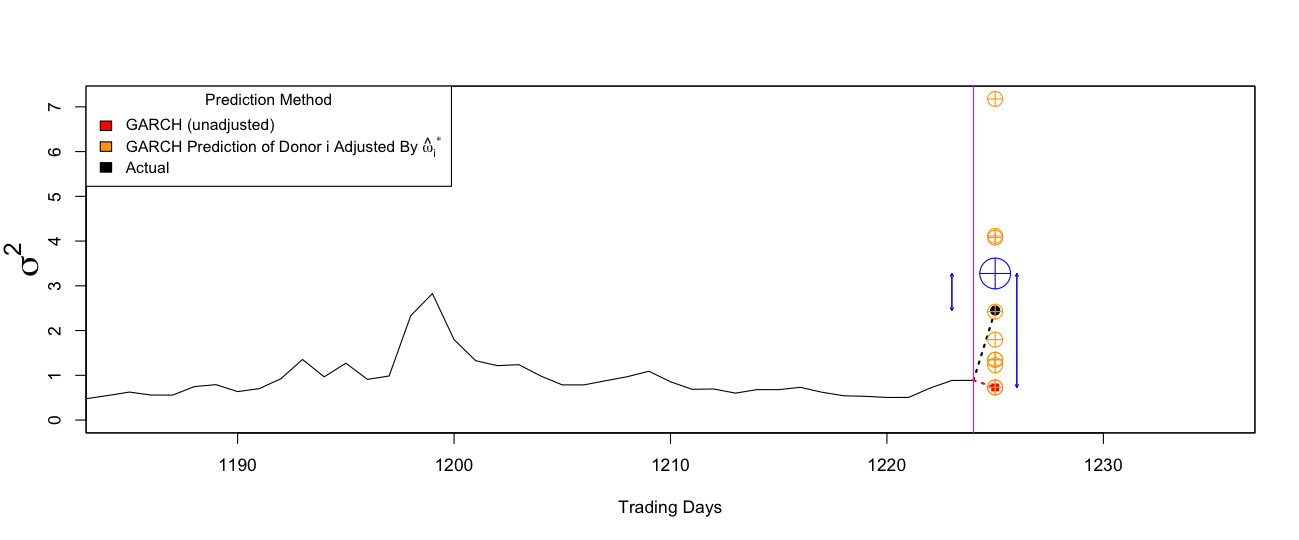
\includegraphics[width=\textwidth]{simulation_plots/motivating_piece_convex_combination.png}};
        % \draw[red,ultra thick,rounded corners] (7.5,5.3) rectangle (9.4,6.2);
        % \node[draw,text width=4.45cm] at (9.8,3.2) {$\textcolor{blue}{\hat\sigma^{2}_{adjusted} = \hat\sigma^{2}_{unadjusted} + \hat\omega^{*}}$ };
        % \node[draw,text width=2.62cm] at (14.8,2.8) {$\textcolor{blue}{\hat\omega^{*} = \sum^{n+1}_{i=2}\pi_{i}\hat\omega^{*}_{i}}$ };    
        
    \end{tikzpicture}
      \caption{The simulated time series experiences a volatility shock between trading days 1,656 and 1,657.  The GARCH prediction, in red, fails even to approach the volatility spike at $T^{*}+1$, as do several adjusted predictions, which are orange.  In contrast, the GARCH forecast adjusted by $\hat\omega^{*} = \sum^{n+1}_{i=2}\pi_{i}\hat\omega^{*}_{i} $, a convex combination of the estimated shocks in the donor pool, achieves directional correctness as well as a smaller absolute loss in its prediction.  The pink vertical line serves to indicate the adjustment of size $\hat\omega^{*}$ that allows the blue bullseye to approach more closely the ground truth.}    
      \label{fig:motivating_piece_convex_combination}
   
      \end{center}
    \end{figure}

  \subsection{A Primer on GARCH}
We define the log return of an asset between $t-1$ and $t$ as $r_{t} = \text{log}(\frac{P_{t}}{P_{t-1}})$, where $P_{t}$ denotes the price at time $t$.  The class of ARIMA($p,d,q$) models  \parencite[][]{box2013box} provides a framework for modeling the autoregressive structure of $r_{t}$.  These models assume a certain dependence structure between $r_{t}$ and $(r_{k})_{k\leq t}$, yet their errors --- often called innovations in the financial time series context due to how they represent the impact of new information --- are nevertheless assumed to be i.i.d. with mean zero and constant variance.  The ARCH \parencite[][]{engle1982autoregressive} and GARCH \parencite[][]{bollerslev1986generalized} models provide elegant alternatives to the homoskedasticity assumption.  In fact, the GARCH framework in its most basic form disregards $r_{t}$ and instead turns its interest to the series $r_{t}^{2}$ (once properly centered, i.e. after assuming a mean-model for returns).  

To that end, let $a_{t} = r_{t} - \mu_{t}$, where $\mu_{t}$ is the (potentially time-varying) mean of the log return series $r_{t}$.  

We thus derive a mean-zero process $(a_{t})_{t\in\mathbb{N}}$ with the property that $\E[a^{2}_{t}] = \mrm{Var}[a_{t}]$.  Under the assumption of time-invariant volatility, the series $a_{t}^{2}$ should exhibit no significant autocorrelation at any lag $\ell\geq1$.  This assumption motivates tests for ARCH effects, that is, tests for the clustering of volatility.  These tests explore the alternative hypothesis that $\sigma_{t}^{2}$ is not only a time-varying parameter but furthermore a function of past squared residuals of the mean model.  In particular, the ARCH($m$) model is an autoregressive model in which $\sigma_{t}^{2}$ is a deterministic function of the past $m$ values of $r_{t}^{2}$.  The GARCH($m,s$) framework take this one step further by modeling $\sigma_{t}^{2}$ as a linear combination of the past $m$ values of $r_{t}^{2}$ and well as the past $s$ values of $\sigma_{t}^{2}$.  In functional form, a GARCH process (sometimes called a strong GARCH process \parencite[][][p. 19]{francq2019garch}) is given by

\begin{align*}
&\sigma_{t}^{2} = \omega + \sum^{m}_{k=1}\alpha_{k}a^{2}_{t-k} + \sum_{j=1}^{s}\beta_{j}\sigma_{t-j}^{2}\\
&a_{t} = \sigma_{t}\epsilon_{t}\\
&\epsilon_{t} \simiid E[\epsilon_{t}]=0, Var[\epsilon_{t}] = 1\\
&\forall k,j, \alpha_{k},\beta_{j}\geq 0\\ 
&\forall t, \omega, \sigma_{t} > 0 \text { .} 
\end{align*}
Assuming further that $\sigma^{2}_{t}$ depends on a vector of exogenous covariates $\x_{t}$, we have a  GARCH-X$(m,s)$.  The volatility equation then becomes 

\begin{align}
\sigma_{t}^{2} = \omega+ \sum^{m}_{k=1}\alpha_{k}a^{2}_{t-k} + \sum_{j=1}^{s}\beta_{j}\sigma_{t-j}^{2} + \gamma^{T}\x_{t} \text{ .}\label{GARCH-X}
\end{align}

\subsection{Model setup}
\label{modelsetup}
We will suppose that a researcher has multivariate time series data $\y_{i,t} = (r_{i,t}$, $\x_{i,t}$), $t = 1,$ $\ldots,  T_i$, $i = 1, \ldots, n+1$, where $r_{i,t}$ is scalar and $\x_{i,t}$ is a vector of covariates such that $\x_{i,t}|\mathcal{F}_{i,t-1}$ is deterministic.  Suppose that the analyst is interested in forecasting the volatility of $r_{1,t}$, the first time series in the collection, which we will denote \textit{the time series under study}.  We require that each time series $\y_{i,t}$ is subject to an observed news event following $T^*_i \leq T_{i} + 1$ and before witnessing $T^*_i+1$.  We are implicitly leveraging the fact that financial assets are heavily-traded during market hours, yet only thinly traded (if traded at all) outside market hours.  In contrast, the arrival of market-moving news does not obey any such restrictions.  In light of the foregoing, we can denote our collection of GARCH-X volatility equations of interest using the following notation

\begin{align*}
&\sigma_{i,t}^{2} = \omega_{i} + \sum^{m_{i}}_{k=1}\alpha_{i,k}a^{2}_{i,t-k} + \sum_{j=1}^{s_{i}}\beta_{i,j}\sigma_{i,t-j}^{2} + \gamma_{i}^{T} \x_{i,t} \text{ }. \\
\end{align*}
Let $I(\cdot)$ be an indicator function.  Let $T_i$ denote the time length of the time series $i$ for $i = 1, \ldots, n+1$, and let $T_i^*$ denote the largest time index prior to the arrival of the news shock, with $T_i^* < T_i$, to ensure that there is at least one post-shock realization for each series $i$.  Let $\delta, \x_{i,t} \in \mathbb{R}^{p}$.  Let $\mathcal{F}_{i}$ with a single-variable subscript denote a univariate, time-invariant $\sigma$-algebra, and $\mathcal{F}_{i,t}$ denote the canonical product filtration for donor $i$ at time $t$.  Let $D^{return}_{i,t} = I(t \in \{T_i^* + 1,...,T_i^* + L_{i, return}\})$ and $D^{vol}_{i,t} = I(t \in \{T_i^* + 1,...,T_i^* + L_{i, vol}\})$, and let $L_{i,return},L_{i,vol}$ denote the lengths of the level and volatility shocks, respectively.  For $t= 1, \ldots, T_i$ and $i = 1, \ldots, n+1$, the model $\mc{M}_1$ is defined as 
\begin{align*}
  \mc{M}_1 \colon \begin{array}{l}
     \sigma^{2}_{i,t} = \omega_{i} + \sum^{m_{i}}_{k=1}\alpha_{i,k}a^{2}_{i,t-k} + \sum_{j=1}^{s_{i}}\beta_{i,j}\sigma_{i,t-j}^{2} + \gamma_{i}^{T} \x_{i,t} + \omega^{*}_{i,t}, \text{ }\\[.2cm]
     a_{i,t} = \sigma_{i,t}((1-D^{return}_{i,t})\epsilon_{i,t} + D^{return}_{i,t}\epsilon^{*}_{i}),\\[.2cm]
    \omega_{i,t}^{*} = D^{vol}_{i,t}[\mu_{\omega^{*}}+\delta^{T}\x_{i,T^{*}_{i}+1}+ u_{i,t}],
  \end{array}
  \end{align*}

with time-invariant error structure
  \begin{align*}
    \epsilon_{i,t} &\simiid \mc{F}_{\epsilon} \text{ with}  \; \mrm{E}_{\mc{F}_{\epsilon}}(\epsilon) = 0, \mrm{Var}_{\mc{F}_{\epsilon}}(\epsilon)  = 1,  \\
    \epsilon^{*}_{i,t} &\simiid \mc{F}_{\epsilon^{*}} \text{ with}  \; \mrm{E}_{\mc{F}_{\epsilon^{*}}}(\epsilon) = \mu_{\epsilon^{*}}, \mrm{Var}_{\mc{F}_{\epsilon^{*}}}(\epsilon^{*})  = \sigma^2_{\epsilon^{*}},  \\
    u_{i,t} & \simiid  \mc{F}_{u} \text{ with}  \; \mrm{Var}_{\mc{F}_{u}}(u) = \sigma^2_{u},\\
    \epsilon_{i,t} & \indep  \epsilon^{*}_{i,t}  \indep u_{i,t}.
    \end{align*}

    Let $\mc{M}_{0}$ denote the subclass of $\mc{M}_{1}$ models such that $\delta \equiv 0$.  Note that $\mc{M}_{0}$ assumes that nonzero shocks have no dependence on the covariates and are i.i.d. with $\E[ \omega^{*}_{i,t}]=\mu_{\omega^{*}}$, where the lack of indices $i$ or $t$ on $\mu_{\omega^{*}}$ indicates that it is shared across donors and is time-invariant. Models $\mc{M}_{1}$ and $\mc{M}_{0}$ parameterize changing dynamics after a shock is observed (when $t \geq T_i^*+1$ for each series $i$). It is important to note that our modeling setup will additionally suppose that $\x_{i,t}$ will be observed before $\sigma_{i,t}^2$ is observed. 
    
Note also the divergences from \cite{lin2021minimizing}.  As already established, the model presented here is intended to account for ARCH effects.  Additionally, here we also diverge by modeling the shocks $\omega^{*}_{i,t}$ as time-varying quantities obeying a mixture distribution.  In particular, prior to and after the shock, the  $\omega^{*}_{i,t}$  are uniformly zero.  During the shock, i.e. from $T^{*}_{i}+1$ through $T^{*}_{i}+L^{vol}_{i}$, the $\omega^{*}_{i,t}$ are distributed i.i.d, with a core signal component that depends solely on the unknown parameter $\delta$ and the observable vector $\x_{i,T_{i}^{*}+1}$.  Wherever necessary, to distinguish the two distributions that make up the shock distribution, we use the term \textit{nonzero shocks} to refer to the shocks that are not uniformly zero.  

The nonzero shocks each include an idiosyncratic noise term that varies across time and donors.  This feature allows the nonzero shocks to exhibit some variation as the shock progresses, even within a single donor.  The noise term could be modeled with additional complexity, including serial correlation, or could exhibit deterministic or stochastic decay throughout the shock period, proportional to a deterministic or stochastic function of time, or could peak somewhere in the middle of the shock period.  Each of these ideas might correspond to some particular, realistic feature of the world.

The model $\mc{M}_1$ is defined by a volatility equation and mean equation, as is any GARCH model.  The decision to model the volatility shock $\omega^{*}_{i,t}$ as an additive random effect is consistent with our setup.  However, the decision to model the level effect $\epsilon^{*}_{i,t}$ as a temporary rupture in the otherwise i.i.d. sequence of innovations $\epsilon_{i,t}$ may not be intuitive.  One way of arguing for this choice is that, in a discrete time series model, if we assume the arrival of news in the time between $T_{i}^{*}$ and $T_{i}^{*}+1$, we do not have an easy way to express a conditional distribution of the innovation $\epsilon_{i,T_{i}^{*}+1}$ given the arrival of information.  Using $\epsilon^{*}_{i,t}$ thus breaks this impasse.  This justification also explains why we do not parameterize the level shock at $T_{i}^{*}+1$ as a sum of two shocks, $\epsilon_{i,T_{i}^{*}+1}$ and $\epsilon^{*}_{i,T_{i}^{*}+1}$, which would represent the level shock as generated by two independent sources of stochasticity. While we want to model the level shocks at $T_{i}^{*}+1$ as potentially large in absolute value, we also want to retain the property of a unitary source of noise.


\section{Methodology for Similarity-based Parameter Correction}

We now introduce how a researcher can carry out predictions via distance-based weighting.  The first step is to gather the $p$ covariates that will parametrize a change in dynamics to model $\mc{M}_1$ and will represent the $p$-dimensional space in which weights are generated.  This set of covariates parameterizes the shock to $\sigma^2_{i,t}$  of magnitude $\omega^*_{i,t}$ in model $\mc{M}_{1}$ above.  Let $\textbf{V}_{t} \in \mathbb{R}^{p \times n}$ be formed with columns $\x_{i,t}$, $i = 2,\ldots,n+1$.  Without loss or generality, let the indices of each $\x_{i,t}$ be shifted and arranged such that $\textbf{V}_{T^{*}+1}$ has as columns $\x_{2,T_{2}^{*}+1},...,\x_{n+1,T_{n+1}^{*}+1}$.  Formally, in vector notation, the donor shocks are given by $\vec{\omega}_t = \vec{\mu}_{\omega^{*}} + \delta^{T}\textbf{V}_{t} + \vec{u}_{t}$, 
    where were have suppressed the $D^{vol}_{i,t}$ notation for simplicity.  %The covariate set could take the form of a $p \times n$ matrix including realized volatility and implied volatility, as well the volume of traded assets on any day preceding the shock.  Covariates chosen for inclusion in a given volatility profile may be levels, log differences in levels, percentage changes in levels, or absolute values thereof, among many choices.
    Ideally, $\textbf{V}_{t}$ will display `balance' in that $p$ covariates exist for each of the $n$ donors.  In practice, missing values, corrupted values, or unacceptably extreme or noisy estimates may necessitate some sort of matrix completion, a problem that we do not tackle in this work.  


    \subsection{Forecasting}\label{two_forecasts}

    We now turn to the next section, where $\textbf{V}_{t}$ is employed in a procedure to arrive at a forecast adjustment. For illustration, we present two one-step-ahead forecasts for the time series under study. The first is the unadjusted GARCH forecast. The second is the adjusted forecast, which differs by the additive term $\hat\omega^{*}$ that is computed via our distance-based weighting procedure.  These forecasts are: 
    
    \begin{align*}
      %\text{Forecast 1: } 
      & \hat\sigma^{2}_{unadjusted,T_{1}^{*}+1} = \hat\E[\sigma^{2}_{1,T_{1}^{*}+1}|\mathcal{F}_{T_{1}^{*}}] && = && \hat\omega_{1} + \sum^{m_{1}}_{k=1}\hat\alpha_{1,k}a^{2}_{1,T_{1}^{*}+1-k} + \sum_{j=1}^{s_{1}}\hat\beta_{1,j}\sigma_{1,T_{1}^{*}+1-j}^{2} + \hat\gamma_{1}^{T} \x_{1,T_{1}^{*}+1},\\
      %\text{Forecast 2: } 
      & \hat\sigma^{2}_{adjusted, T_{1}^{*}+1} = \hat\E[\sigma^{2}_{1,T_{1}^{*}+1}|\mathcal{F}_{T_{1}^{*}}] + \hat\omega^{*} && = && \hat\omega_{1} + \sum^{m_{1}}_{k=1}\hat\alpha_{1,k}a^{2}_{1,T_{1}^{*}+1-k} + \sum_{j=1}^{s_{1}}\hat\beta_{1,j}\sigma_{1,T_{1}^{*}+1-j}^{2} + \hat\gamma_{1}^{T} \x_{1,T_{1}^{*}+1} + \hat\omega^{*} \text{ .}
    \end{align*}
    
    Note that GARCH models can be parameterized as ARMA models on the squares of the scalar time series $a_{i,t}^{2}$ \parencite[][]{tsay2005analysis,francq2019garch}, assuming that $a_{i,t}$ satisfies fourth-order stationarity.  This fact matters for forecasting because the $h$-step-ahead forecasting function for a GARCH model is, just like for an ARMA model, the conditional expectation function, $\mathbb{E}[ \sigma^{2}_{i,T_{i}^{*}+h} | \mathcal{F}_{T_{i}^{*}}]$, or practically speaking, the estimate thereof, $\hat{\mathbb{E}}[ \sigma^{2}_{i,T_{i}^{*}+h} |\mathcal{F}_{T_{i}^{*}}]$ \parencite[][]{zivot2009practical}.  Here we have presented one-step-ahead forecasts for a GARCH-X($m,s$).  For $h=2,3,4,...$, the conditional expectation is computed recursively, as is standard for iterative autoregressive forecasts. Note that $h$-step-ahead predictions will require, of course, some reasonable idea about the length of time for which the adjustment quantity $\hat\omega^{*}$ should be included.  Additionally, if $\x_{1,t}$ is used as an exogenous regressor in order to estimate $\gamma_{1}$ prior to the shock period, then strictly speaking, $\x_{1,t+h}|\mathcal{F}_{t}$ must be deterministic --- at least for the relevant $(t,h)$ pair for which a forecast is sought.   In practice, it may be acceptable for $\x_{1,t+h}|\mathcal{F}_{t}$ to be merely well-estimated. Thus for simplicity of exposition, we will focus on the one-step-ahead forecast unless stated otherwise.

    \subsection{Excess Volatility Estimators}
    \label{Excess Volatility Estimators}
   
    The problem of aggregating estimated donor shocks begins with the data constraints.  Let us first introduce useful notation.  Let $\hat\omega^{*}_{i,*}$ denote the shock estimate for donor $i$ that is obtained via fixed effect estimation over time points $T_{i}^{*}+1,...,T_{i}^{*}+L_{i,vol}$.  That estimation procedure is justified by the assumption that at each nonzero shock point, the shocks will differ but will be equal in distribution.  
    
    Taking the estimated shocks as a given, we observe the pair $(\{\hat\omega^{*}_{i,*}\}^{n+1}_{i=2},\{\textbf{v}_{i}\}^{n+1}_{i=2})$.  Let $\Delta^{n-1} = \{\pi \in \mathbb{R}^n: \sum_{i=1}^n \pi_i = 1, \pi_i \geq 0, i = 1,...,n\}$.  We wish to recover weights $\{\weight_{i}\}^{n+1}_{i=2} \in \Delta^{n-1}$ leading to favorable forecasting properties.  These weights are used to define and compute an aggregate shock estimate 
\begin{equation} \label{adjustment}
	  \hat\omega^{*} = \sum^{n+1}_{i=2}\weight_{i}\hat\omega^{*}_{i,*},
\end{equation}
    which will be taken to be our forecast adjustment term.  Since the weights $\{\weight_{i}\}_{i=2}^{n+1}$ are computed using $\mathcal{F}_{T^{*}_{i}}$, the set $\{\weight_{i}\}_{i=2}^{n+1}$ is deterministic and observed, $\textit{modulo}$ any stochastic ingredient in the numerical methods employed to approximate $\x_{1,T_{1}^{*}+1}$ using a convex combination of donor covariates.  We say more about the properties of the shocks $\omega^{*}_{i,T_{i}^{*}+1},...,\omega^{*}_{i,T_{i}^{*}+L^{vol}_{i}}$ in section $\ref{SVF_properties}$. 

    Following \cite[][]{abadie2003economic},\cite[][]{abadie2010synthetic},\cite[][]{lin2021minimizing}, let $\|\cdot\|_{\textbf{S}}$ denote any semi-norm on $\mathbb{R}^{p}$, and define
    \begin{align*}
    \{\pi\}_{i=2}^{n+1} = \argmin_{\pi}\|\x_{1,T_{1}^* + 1} - \V_{T^* + 1}\pi\|_{\textbf{S}}. 
    \end{align*}
In the forecast combination literature, it is of interest whether the weights employed to aggregate forecasts strive toward and meet various optimality criteria \cite[][]{timmermann2006forecast,wang2023forecast}.  In our endeavor, there are at least two senses of optimal weights that one might be interested in.  First, we can think of optimal weights as a set $\{\weight_{i}\}_{i=2}^{n+1}$ such that $\omega_{1} = \sum^{n+1}_{i=2}\weight_{i}\hat\omega_{i,*}$, i.e., $\omega_{1}$ is recovered perfectly, as it belongs to convex hull of the estimated shocks. However, $\omega_{1}$ is never revealed to the practitioner, and hence there is no way of verifying the extent to which this condition is satisfied.

A more promising aim is finding weights such that $\textbf{v}_{1} = \sum^{n+1}_{i=2}\weight_{i}\textbf{v}_{i,T_{1}^{*}+1}$, meaning that the covariates of the time series under study lies within the convex hull of the donor covariates.  This condition underwrites asymptotic results in \cite[][]{abadie2010synthetic}, and the intuition there extends to this work: if the shock is parameterized by an affine function of covariates, then finding a linear combination that recreates the shock should serve us well.  Because the method proposed uses a point in $\Delta^{n-1}$, it is important to head-off possible confusion.  What we are proposing is not a forecast combination method.  What we are aggregating and weighting (not combining) are subcomponents of forecasts, not forecasts themselves.  Moreover, from a broader perspective, forecast combination is an inapt term for what is being proposed here.  First, the donor time series do not provide forecasts, nor would forecasts be needed for random variables that have already been realized.  Second and more fundamentally, the theoretical underpinnings of forecast combination, while diverse \cite[][]{wang2023forecast}, are distinct from the setting presumed in this work.

Supposing that we can define optimal weights, then uniqueness may still be a concern. \cite[][]{lin2021minimizing} discuss sufficient conditions for uniqueness as well as the implications of non-uniqueness.  \cite[][]{abadie2022synthetic} invoke the Carath\'eodory Theorem to argue for the sparseness of the weight vector.  We make additional comments as well. $(\mathbb{R}^{n}, \|\cdot\|)$ is a Chebyshev space, and hence for any element $x$ and any convex set $C\subset \mathbb{R}^{n}$, there exists a unique element $y\in C$ that minimizes $\|x-y\|$.  However, the pre-image of $y$ with respect to a particular operator and constraint set might not be unique.  Let $p', n'$ denote the number of linearly independent rows of $\V_{t}$ and linearly independent columns of $\V_{t}$, respectively.  Let col($\cdot$) denote the column space of a matrix, and let Conv($\cdot$) denote the convex hull of a set of column vectors. The following table is useful for categorization of when a perfect fit and uniqueness prevail.

    \begin{center}
      \begin{tabular}{ | m{3em} | m{7cm}| m{7cm} | } 
        \hline
        & $\textbf{v}_{1}\in \text{Conv}(\text{col}(\V_{t}))$ & $\textbf{v}_{1} \notin \text{Conv}(\text{col}(\V_{t}))$\\ 
        \hline
        $p' \geq n'$ & Perfect fit; minimizer unique & Fit not perfect; minimizer unique \\
        \hline
        $p' < n'$ & Perfect fit; minimizer not necessarily unique, Carath\'eodory Theorem applies& Fit not perfect; minimizer not necessarily unique, Carath\'eodory Theorem applies \\ 
        \hline
      \end{tabular}
      \end{center}
      
It should be noted, however, that even when the minimizer is unique, finding that unique minimizer may require numerical methods.  In the event that one's preferred numerical optimization routine fails to arrive at a single solution on the simplex in repeated runs of the algorithm, some sort of forecast combination might be advised.  We discuss forecast combination later in this paper in the context of robustifying against misspecification.

On the questions of convex geometry and convex optimization, comparison with least-squares estimation is also illustrative.  Consider least-squares estimation for the $p$-vector $\delta$ in the shocks $\omega^{*}_{i,t}$:

\begin{align*}
 \hat\omega^{*}_{OLS} =\argmin_{\delta}\|\hat{\omega}^{*} - \delta^{T}\textbf{V}_{T^{*}+1}\|^{2}_{2},
\end{align*}
where $\textbf{V}_{T^{*}+1}$ could include an adjoined row $\textbf{1}_{n}$, in order to estimate the locator parameter of the shock.  One problem is that this optimization problem is an optimization problem over $p$-vectors $\delta$ --- over linear combinations of the covariates, whereas what we seek is an $n$-vector --- a linear combination of donors.  Additionally, there is no guarantee that $\hat\omega^{*}_{OLS} = \hat{\delta}_{OLS}^{T}\x_{1,T^{*}+1}$ would perform poorly, but given the small number of donors supposed in our setting, it is risky.  Last, and perhaps most challenging for the least-squares estimate, $\hat{\delta}_{OLS}^{T}$ faces the usual requirement of more donors than linearly independent covariates, and that may not often be easy to satisfy in our setting.

\subsection{Ground Truth Estimators}
    \label{Ground Truth Estimators}
    
    The time-varying parameter $\sigma^{2}_{t}$ is a quantity for which even identifying an observable effect in the real world is far more challenging.  In this work, we use a common estimator of the variance called realized volatility (RV), one which has the virtue of being ``model-free'' in the sense that it requires no modeling assumptions \cite[][]{andersen2010stochastic}.  The realized variance itself can be decomposed into the sum of a continuous component and a jump component, with the latter being less predictable and less persistent \cite[][]{andersen2007roughing}, cited in \cite[][]{de2006forecasting}, two factors that further motivate the method employed herein.
    
    Suppose we examine $K$ units of of time, where each unit is divided into $m$ intervals of length $\frac{1}{m}$.  We adapt the notation of \cite[][]{andersen2008realized}. Let $p_{t} = \log{P_{t}}$, and let $\tilde{r}(t,\frac{1}{m}) = p_{t} - p_{t-\frac{1}{m}}$.  Suppressing the $i$ index, we estimate the variance the log return series using Realized Volatility of the $K$ consecutive trading days that conclude with day $t$, denoted $RV_{t}^{K,m}$, using    
   \begin{align*}
    RV_{t}^{K,m} = \frac{1}{K}\sum^{Km}_{v=1}\tilde{r}^{2}(v/m,1/m),
   \end{align*}
    where the $K$ trading days have been chopped into $Km$ equally-sized blocks.

    Assuming that the $K$ units $\tilde{r}(t, 1) = p_{t} - p_{t-1}$ are such that $\tilde{r}(t, 1) \simiid N(\mu, \delta^{2})$, it is easily verified that $\E[RV^{K,m}] = \frac{\mu^{2}}{m} + \delta^{2}$, which is a biased but consistent estimator of the variance.  We will proceed using $m = 77$, corresponding to the 6.5-hour trading day chopped into 5-minute blocks, with the first block omitted in order to ignore unusual trading behavior at the start of the day. Other sensible choices for $m$ can replace our specification if desired.

\subsection{Loss Functions}\label{loss_function}

We are interested in point forecasts for $\sigma^{2}_{1,T_{1}^{*}+h}|\mathcal{F}_{T_{1}^{*}}$, $h=1,2,...,$ the $h$-step ahead conditional variance for the time series under study.  Let $L^{h}$ with the subscripted pair $\{$prediction method, ground truth estimator$\}$, denote the loss function for an $h$-step-ahead forecast using a given prediction function and ground truth estimator.  For example, the $h$-step-ahead MSE when forecasting from time $t$ using our method and using Realized Volatility as the ground truth is

\begin{align*} 
  \text{MSE}^{h}_{\text{adjusted prediction, RV}} = (\hat\sigma^{2}_{\text{adjusted prediction},t+h} - \hat\sigma^{2}_{RV,t+h})^{2}\text{ .}
\end{align*}
Also of interest in absolute percentage error for an $h$-step-ahead forecast, defined as

\begin{align*}
\text{APE}^{h}_{\text{method, ground truth}} = \frac{|\hat\sigma^{2}_{\text{method},t+h} - \hat\sigma^{2}_{\text{ground truth},t+h}|}{\hat\sigma^{2}_{\text{ground truth},t+h}}\text{ .}
\end{align*}
Finally, we introduce the QL (quasi-likelihood) Loss \cite[][]{brownlees2011practical}:

\begin{align*}
\text{QL}^{h}_{\text{method, ground truth}} = \frac{\hat\sigma^{2}_{\text{ground truth},t+h}}{ \hat\sigma^{2}_{\text{method},t+h}} - \log{\frac{\hat\sigma^{2}_{\text{ground truth},t+h}}{ \hat\sigma^{2}_{\text{method},t+h}}} -1 \text{ .}
\end{align*}
What distinguishes QL Loss is that it is multiplicative rather than additive.  This has benefits, both practical and theoretical.  As \cite[][]{brownlees2011practical} explain, the technical properties of the QL Loss allow researchers to compare forecasts across heterogeneous time series, whereas additive loss functions like MSE unfairly penalize forecasts made under market turbulence.  For this reason and others, we proceed to evaluate the method, both in simulations and real data examples, using the QL loss.

\section{Properties of Volatility Shocks and Shock Estimators}\label{SVF_properties}

In this section we will provide estimation properties for our shock  estimator \eqref{adjustment} and our adjusted forecast. These results will be with $m_i = s_i = 1$, for all $i = 1,\ldots,n+1$ in model $\mc{M}_1$ unless otherwise stated, i.e. a GARCH(1,1) model with additional parameterizations for shocks. Note that the dual level-volatility shock in $\mc{M}_1$ has a marginal effect on the conditional variance $\sigma^{2}_{i,t}$ that reflects the geometric decay of innovations in autoregressive models.  As usual, assume $\alpha+\beta < 1$.  Furthermore, assume that both the volatility shock and the level shock are of length one only, and consider a circumstance with no exogenous covariate $\x_{i,t}$, except in the conditional shock distribution. Assume also that $r\geq 2$, which is necessary in order to isolate the effects of the level shock $\epsilon^{*}_{i,t}$.  Then
\begin{align}
\sigma^{2}_{i,T_{i}^{*}+r+1} | \mathcal{F}_{T_{i}^{*}+r} & = \omega_{i} + \alpha_{i} a_{T_{i}^{*}+r}^{2} + \beta_{i}\sigma^{2}_{i,T_{i}^{*}+r} \label{eq0}\\
& = \omega_{i} + \alpha_{i}(\sigma_{i,T_{i}^{*}+r}\epsilon_{T_{i}^{*}+r})^{2} + \beta_{i}\sigma^{2}_{i,T_{i}^{*}+r}\notag \\
& = \omega_{i} + \sigma^{2}_{i,T_{i}^{*}+r}(\alpha_{i} (\epsilon_{T_{i}^{*}+r})^{2} + \beta_{i}) \text{ .}\notag 
\end{align}

In Equation \eqref{eq0}, observe that $\omega_{i,T_{i}^{*}+1}^{*}$ and $\epsilon^{*}_{i,T_{i}^{*}+1}$ 
each appear at most once, through the term $\sigma^{2}_{T_{i}^{*}+r}$.  This might lead one to 
suspect  geometric decay of the shocks $\omega_{i,T_{i}^{*}+1}^{*}$ and $\epsilon^{*}_{i,T_{i}^{*}+1}$.  
Such a suspicion is easier to justify by examining the conditional expectation of the variance, 
$\mathbb{E}[ \sigma^{2}_{i,T_{i}^{*}+r+1} |\mathcal{F}_{T_{i}^{*}+r}]$, which also happens to be the principal forecasting tool for a GARCH model \cite[][]{zivot2009practical}.  Indeed, if we assume unit variance for all $\epsilon_{i,t}$ except, of course, $\epsilon^{*}_{i,t}$, then we have

\begin{align*}
\mathbb{E}[ \sigma^{2}_{i,T_{i}^{*}+r+1} |\mathcal{F}_{T_{i}^{*}+r}] & = \mathbb{E}[\omega_{i} + \alpha a_{T_{i}^{*}+r}^{2} + \beta\sigma^{2}_{i,T_{i}^{*}+r} |\mathcal{F}_{T_{i}^{*}+r}] \\
& = \omega_{i} + \mathbb{E}[\alpha(\sigma_{i,T_{i}^{*}+r}\epsilon_{T_{i}^{*}+r})^{2} |\mathcal{F}_{T_{i}^{*}+r}] + \beta\sigma^{2}_{i,T_{i}^{*}+r} \\
& = \omega_{i} + \alpha\sigma_{i,T_{i}^{*}+r}^{2} + \beta\sigma^{2}_{i,T_{i}^{*}+r} \tag{Due to the unit variance assumption}\\
& = \omega_{i} + \sigma^{2}_{i,T_{i}^{*}+r}(\alpha + \beta) \text{ .} 
\end{align*}
By repeated substitution, in conditional expectation, the shock belongs to the equivalence class $\mathcal{O}((\alpha+\beta)^{r})$.  We generalize this observation in the following proposition.

\begin{prop}\label{decay_prop}
Let $a_{i,t}$ be a mean-zero time series obeying a GARCH(1,1) specification with unit-variance errors, all prior to the arrival of a volatility shock of length $L_{i}^{vol} \geq 1$ and level shock of length $L_{i}^{return}\geq 1$ at some time $T_{i}^{*}+1$.  Then for any $i$, $1\leq i \leq n+1$, and $r$ such that $r \geq \text{max}\{L_{i}^{return},L_{i}^{return}\} + 1$, 
\begin{align*}
\mathbb{E}[ \sigma^{2}_{i,T_{i}^{*}+r+1} |\mathcal{F}_{T_{i}^{*}+r}] & = \omega_{i} + (\alpha + \beta)\sigma^{2}_{i,T_{i}^{*}+r}.
\end{align*}
\end{prop}

In other words, for a GARCH(1,1), once two time points removed from the longest shock length, the volatility shock and level shock can be subsumed into one.  However, prior to being two time points removed, there is no such guarantee.  For example, one can take $r = 1$ and level shock of length at least 1 to see that 

\begin{align*}
\mathbb{E}[ \sigma^{2}_{i,T_{i}^{*}+2} |\mathcal{F}_{T_{i}^{*}+1}] & = \mathbb{E}[\omega_{i} + \alpha a_{T_{i}^{*}+1}^{2} + \beta\sigma^{2}_{i,T_{i}^{*}+1} |\mathcal{F}_{T_{i}^{*}+1}] \\
& = \omega_{i} + \mathbb{E}[\alpha(\sigma_{i,T_{i}^{*}+r}\epsilon^{*}_{T^{*}+1})^{2} |\mathcal{F}_{T_{i}^{*}+1}] + \beta\sigma^{2}_{i,T_{i}^{*}+1} \\
& = \omega_{i} + \alpha\sigma^{2}_{i,T_{i}^{*}+1}(\mu^{2}_{\epsilon^{*}} + \sigma^{2}_{\epsilon^{*}}) + \beta\sigma^{2}_{i,T_{i}^{*}+1} \\
& = \omega_{i} + \sigma^{2}_{i,T_{i}^{*}+1}(\alpha(\mu^{2}_{\epsilon^{*}} + \sigma^{2}_{\epsilon^{*}}) + \beta)\text{,}
\end{align*}
where $(\alpha(\mu^{2}_{\epsilon^{*}} + \sigma^{2}_{\epsilon^{*}}) + \beta)$ may be greater than 1, permitting explosive behavior, at least in the short term.  After both shocks have been exhausted, their influence disappears quickly.  This short-memory effect has implications for the method being developed herein.  First, there may be different risks associated with overestimating and underestimating level shock and volatility shock lengths.  Therefore, estimation of effects among the donors should err on the side of underestimating, not overestimating, the length of the max shock, since overestimation of the shock length brings with it the risk of underestimating $\omega^{*}_{i,t}$.  Second, a practitioner of the method needs some idea of how long the the respective shocks in the time series under study might last.  There are couple of obvious strategies: take all the donors, and over all the donor shock lengths, take the minimium.  Alternatively, one could take the maximum.

\subsection{Consistency of the shock estimators}

The estimators $\hat\omega^{*}_{i,t}$ in \eqref{adjustment} are central to our forecast adjustment strategy.  Here we show that the quantities $\hat\omega^{*}_{i,t}$ possess an important asymptotic property that bolsters that overall reliability of the method proposed herein.

\begin{prop}\label{omega_consistency}
Assume
\begin{enumerate}
  \item For each $i$, $1\leq i \leq n$, $\{a_{i,t}\}_{t=0,...,T_i}$ obeys a GARCH-X($m,s$), as laid out in Equation $\eqref{GARCH-X}$, with volatility shocks found in $\mc{M}_{1}$, where $T_i$ is the length of the $i$th series.
  \item For each $i, \{\omega_{i,t}^{*}\}_{t=0,...,T_i}$ is potentially non-zero at $\{T^{*}_{i}+1,... ,T^{*}_{i}+L_{i}^{vol}\}$, $\omega_{i,T_{i}^{*}+1}^{*}\equiv...\equiv\omega_{i,T_{i}^{*}+L_{i}^{vol}}^{*}$, and zero otherwise, where the arrival of $T_{i}^{*}$ is governed by a time-invariant distribution on $\{a_{i,t}\}_{t=0,...,T_i-1}$, and both the arrival and conclusion of the shock is observable by the researcher. \label{stationarity_of_omega_i_t}
  \item The conditions in Assumption 0 of \cite[][]{han2014asymptotic} hold.
\end{enumerate}

Then for any $i, 1\leq i \leq n+1$, and for any $r, 1\leq r \leq L_{i}^{vol}$, $\hat\omega_{i,T_{i}^{*}+r}^{*} \overset{p}{\longrightarrow} \omega_{i,T_{i}^{*}+r}^{*}$ as $t\rightarrow\infty$.  Additionally, $\hat\omega_{i,*}^{*} \overset{d}{\longrightarrow} \omega_{i,T_{i}^{*}+r}^{*}$ as $t\rightarrow\infty$, and if for all $i, 1 \leq i \leq n+ 1$, $u_{i,t} \equiv 0$ on $\{T^{*}_{i}+1,... ,T^{*}_{i}+L_{i}^{vol}\}$, then $\hat\omega_{i,T_{i}^{*}+r}^{*} \overset{p}{\longrightarrow} \omega_{i,T_{i}^{*}+r}^{*}$ .
\end{prop}

\begin{lem}\label{lemma_ref}
  Under assumption \ref{stationarity_of_omega_i_t}, for each $i, i=1,...,n+1$,  $\{\omega_{i,t}^{*}\}_{t=0,...,T_i}$ is a strictly stationary series.
\end{lem}


\subsection{Consistency of the Conditional Forecast Function}

Having established the consistency of the estimators $\hat\omega^{*}_{i,T_{i}^{*}+r}$, we extend that result to prove asymptotic properties of the conditional forecast function itself.

  \begin{prop}\label{sigma_consistency}
    Assume
    \begin{enumerate}
      \item All conditions listed in Proposition \ref{omega_consistency}.
      \item There exist weights $\{\pi_{i}\}_{i=2}^{n+1}$ such that $\textbf{v}_{1,T_{1}^{*}} = \sum^{n+1}_{i=2}\weight_{i} \textbf{v}_{i,T_{i}^{*}}$.
     \end{enumerate}
  Then for any $r$, $1\leq r \leq L_{1}^{vol}$, $\hat\sigma^{2}_{adjusted,T_{1}^{*}+r}\overset{d}{\longrightarrow}\sigma^{2}_{1,T_{1}^{*}+r}$ as $t\rightarrow\infty$ in the donor pool, and if for all $i, 1 \leq i \leq n+ 1$, $u_{i,t} \equiv 0$ on $\{T^{*}_{i}+1,... ,T^{*}_{i}+L_{i}^{vol}\}$, then $\hat\sigma^{2}_{adjusted,T_{1}^{*}+r}\overset{p}{\longrightarrow}\sigma^{2}_{1,T_{1}^{*}+r}$.
  \end{prop}

\subsection{Asymptotic Loss}

We now evaluate the loss and risk of our method under two scenarios: first, under arbitrary distribution of $\sigma^{2}_{t+1}$, and then second, under the assumption that the data-generating process is correctly specified.  We proceed with the same notation for adjusted and unadjusted forecasts introduced in Section \ref{two_forecasts}.  For a 1-step-ahead forecast of $\sigma^{2}_{t+1}$ where $t=T^{*}$, consider the difference 
\begin{align}
  & QL(\hat\sigma_{unadjusted,t+1}^{2},\sigma^{2}_{t+1})-QL(\hat\sigma^{2}_{adjusted,t+1},\sigma^{2}_{t+1})\notag \\
   & =(\frac{\sigma_{t+1}^{2}}{\hat\sigma^{2}_{unadjusted,t+1}} - \log{\frac{\sigma_{t+1}^{2}}{\hat\sigma^{2}_{unadjusted,t+1}} } - 1) - (\frac{\sigma_{t+1}^{2}}{\hat\sigma^{2}_{adjusted,t+1}} - \log{\frac{\sigma_{t+1}^{2}}{\hat\sigma^{2}_{adjusted,t+1}}} - 1)\notag\\
   & = \frac{\sigma_{t+1}^{2}}{\hat\sigma^{2}_{unadjusted,t+1}} - \frac{\sigma_{t+1}^{2}}{\hat\sigma^{2}_{adjusted,t+1}}+ \log{\frac{\hat\sigma^{2}_{unadjusted,t+1}}{\hat\sigma^{2}_{adjusted,t+1}}}\notag\\
   & = \frac{\sigma_{t+1}^{2}(\hat\sigma^{2}_{adjusted,t+1}-\hat\sigma^{2}_{unadjusted,t+1})}{\hat\sigma^{2}_{adjusted,t+1}\hat\sigma^{2}_{unadjusted,t+1}} + \log{\frac{\hat\sigma^{2}_{unadjusted,t+1}}{\hat\sigma^{2}_{adjusted,t+1}}}\label{QL Loss toy example} \text{ .}
\end{align}
For simplicity, we work with a GARCH(1,1) that experiences a volatility shock at a single time point for which we would like to provide a point forecast.  Then (\ref{QL Loss toy example}) can be expressed as
\begin{align*}
   &\frac{\sigma^{2}_{t+1}\hat\omega^{*}_{t+1} }{\hat\sigma^{2}_{adjusted,t+1}\hat\sigma^{2}_{unadjusted,t+1}} + \log{\frac{\hat\omega + \hat\alpha a_{t}^{2} + \hat\beta\sigma_{t}^{2}}{\hat\omega + \hat\alpha a_{t}^{2} + \hat\beta\sigma_{t}^{2} + \hat\omega^{*}_{t+1}}}.
\end{align*}\label{QL Loss Consistency - GARCH(1,1)}
It is easily verified that as $\hat\omega^{*}_{t+1} \rightarrow 0^{+}$, the difference in the losses goes to zero.  On the other hand, as $\hat\omega^{*}_{t+1}$ becomes large, the difference in the losses turns negative, with the lesson being that $\hat\omega^{*}_{t+1}$ must be in appropriate proportion to $\sigma^{2}_{t+1}$ in order for the adjusted forecast to outperform the unadjusted forecast.  This explains why it is so important to avoid using a naive adjustment estimator, $\overline{\omega^{*}}$, the arithmetic mean of the estimated shocks.  We conclude this section with a broader result. 

\begin{prop}\label{asymptotic_consistency}
Assume the conditions in Propositions $\ref{omega_consistency}$ and $\ref{sigma_consistency}$.  Then as $t\rightarrow \infty$ in the donor pool,
$$QL(\hat\sigma_{unadjusted,T^{*}+1}^{2},\sigma^{2}_{T^{*}+1})-QL(\hat\sigma^{2}_{adjusted,T^{*}+1},\sigma^{2}_{T^{*}+1}) \overset{d}{\longrightarrow} \frac{\omega_{1,T^{*}+1}^{*}}{\sigma^{2}_{1,T^{*}+1}-\omega_{1,T^{*}+1}^{*}} + \log{\frac{\sigma_{1,T^{*}+1}^{2}-\omega_{1,T^{*}+1}^{*}}{\sigma_{1,T^{*}+1}^{2}} } \geq 0,$$ and if for all $i, 1 \leq i \leq n+ 1$, $u_{i,t} \equiv 0$ on $\{T^{*}_{i}+1,... ,T^{*}_{i}+L_{i}^{vol}\}$, the convergence is in probability.  Hence, a correctly specified $\mc{M}_1$ model will outperform the unadjusted forecast asymptotically.
\end{prop}

\section{Numerical Examples}

In this section, we demonstrate the effectiveness of the proposed method using Monte Carlo simulations.  All simulations will use $\mc{M}_1$ volatility models and $\mc{M}_0$ models on the returns, i.e. $  D^{return}_{i,t} \equiv 0$ for each $i$ and each $t$.  We first explain the parameters to be varied, the parameters that remain fixed, and the behavior we expect to observe.  For our purposes, a parameter is defined to be fixed whenever it does not vary across any of the simulations performed, and conversely, a parameter is varying whenever it varies across at least two simulations performed. The overarching story told by the simulations is that our method performs well as the magnitude of the signal in the shock grows relative to the variance of the idiosyncratic noise term of the shock. 
%For brevity, we refer to this as the signal-to-noise phenomenon.  However, this phenomenon is complicated somewhat by at least two nuances: additional parameters must be in place and properly sized in order to enable to signal-to-noise phenomenon, and second, certain hurdles must be met in the size of those additional parameters before the signal-to-noise story can be seen.  In short, interaction effects abound, with non-linearities as well.

  \subsection{Fixed Parameters}
Each simulation, $i=1,...n+1$ is a GARCH(1,1) process of length $T_{i}$ chosen randomly from the set of integers $\{756,...,2520\}$, corresponding to approximately 3-10 years of daily financial data.  We fixed the intercept of the processes at the $\textit{garchx}$ package default of $\omega = .2$ \citep{RePEc:pra:mprapa:100301}.  We also use the values $\alpha=.1, \beta = .82$, corresponding to a GARCH process with greater influence from past values of $\sigma^{2}_{i,t}$ than past values of $a^{2}_{i,t}$.


  \subsection{Varying Parameters}
  We vary exactly five parameters: $\mu_{V}, \sigma_{V}, \mu_{\delta}, \mu_{\omega^{*}}, \sigma_{u}$, each of which is critical to evaluating the method's responsiveness to changing conditions in the shock distribution. $\mu_{V}, \sigma_{V}$ govern the elements of the covariates. $\mu_{\delta}$ interacts with $\textbf{V}_{t}$ via the dot-product operation, of course.  $\mu_{\omega^{*}}$ is a location parameter for the volatility shock, and $\sigma_{u}$ is the standard deviation of the volatility shock.
  
  We add an important note about the parameter $\mu_{\delta}$, which governs a vector $\delta$ of length $p$ with elements that increase monotonically in proportion to $1,...,p$, after which they are scaled by the factor $\frac{2\cdot\mu_{\delta}}{p(p+1)}$, so that a randomly selected entry of the vector has mean $\mu_{\delta}$.  The heterogeneity of the entries in $\delta$ is critical to simulating the plausible heterogeneity that will exist in the random effects structure.  Absent a heterogeneous vector $\delta$, the shock would not vary systematically with regard to each variable in the covariate vector.  Such a setup would fail to approximate the realities of financial markets.

\subsection{Evaluative Framework and Monte Carlo Results}
Consistent with our evaluative framework declared in \ref{loss_function}, we compare adjusted and unadjusted forecasts using QL Loss, calculating the fraction of the simulations in which the adjusted forecast yields a QL Loss no smaller than that of the unadjusted forecast.  The simulations fall into three broad categories, which we will denote \textbf{Signal and Noise} (displayed in Figure \ref{fig:signoise}), \textbf{Interaction between Signal and Volatility Profile Means} (displayed in Figure \ref{fig:sig_volprof}), and lastly, \textbf{Interaction between Shock Intercept and Shock Noise} (displayed in Figure \ref{fig:intercept_noise}).  

The first category plots two parameters of the shock equation, $\mu_{\delta}$ and $\sigma_{u}$, in grids while increasing the mean of the covariate vectors $\x$ over three plots.  Recall that $\delta$ is a parameter shared between donors, whereas each vector $\x_{i,t}$ in $\V_{i,t}$ is i.i.d. multivariate normal.  In Figure \ref{fig:sim_1}, we see very little variation across the grid.  However, in Figures \ref{fig:sim_2} and \ref{fig:sim_3}, where $\mu_{v}$ is increased, we observe an expected phenomenon: for any fixed column of the plots, the performance of the adjusted forecast improves with increasing $\mu_{\delta}$.  A somewhat subtler phenomenon is also observed: for a fixed row of the grids in Figures \ref{fig:sim_2} and \ref{fig:sim_3}, for $\mu_{\delta} \geq .5$, increasing $\sigma_{u}$ leads to a decline in performance.  However, this is not observed for smaller levels of $\mu_{\delta}$, where the signal is too weak.

The second category of simulations examines $\mu_{\delta}$ and $\mu_{v}$, while increasing the noise $\sigma_{u}$.  The row-wise and column-wise increases in performance that we witnessed in the first category largely hold in the second category of simulations, with one similar disclaimer: the relationship is strained under large levels of noise, like $\sigma_{u} = 1$.

Lastly, the third set of simulations takes a look at the role of the intercept of the conditional shock distribution, $\mu_{\omega^{*}}$, in particular, its interaction with $\sigma_{u}$.  We can think of $\mu_{\omega^{*}}$ as being the sole component of $\x$ that has no variance, i.e. because its corresponding entry in the vector $\x$ is the scalar 1.  For larger values of $\mu_{\omega^{*}}$, the outperformance of the adjusted forecast declines with increases in $\sigma_{u}$, but this effect is absent for smaller values of $\mu_{\omega^{*}}$ 

    \begin{figure}[!h]
      \centering
      \textbf{Signal and Noise}\par\medskip
    \begin{subfigure}{.44\linewidth} 
      \centering
        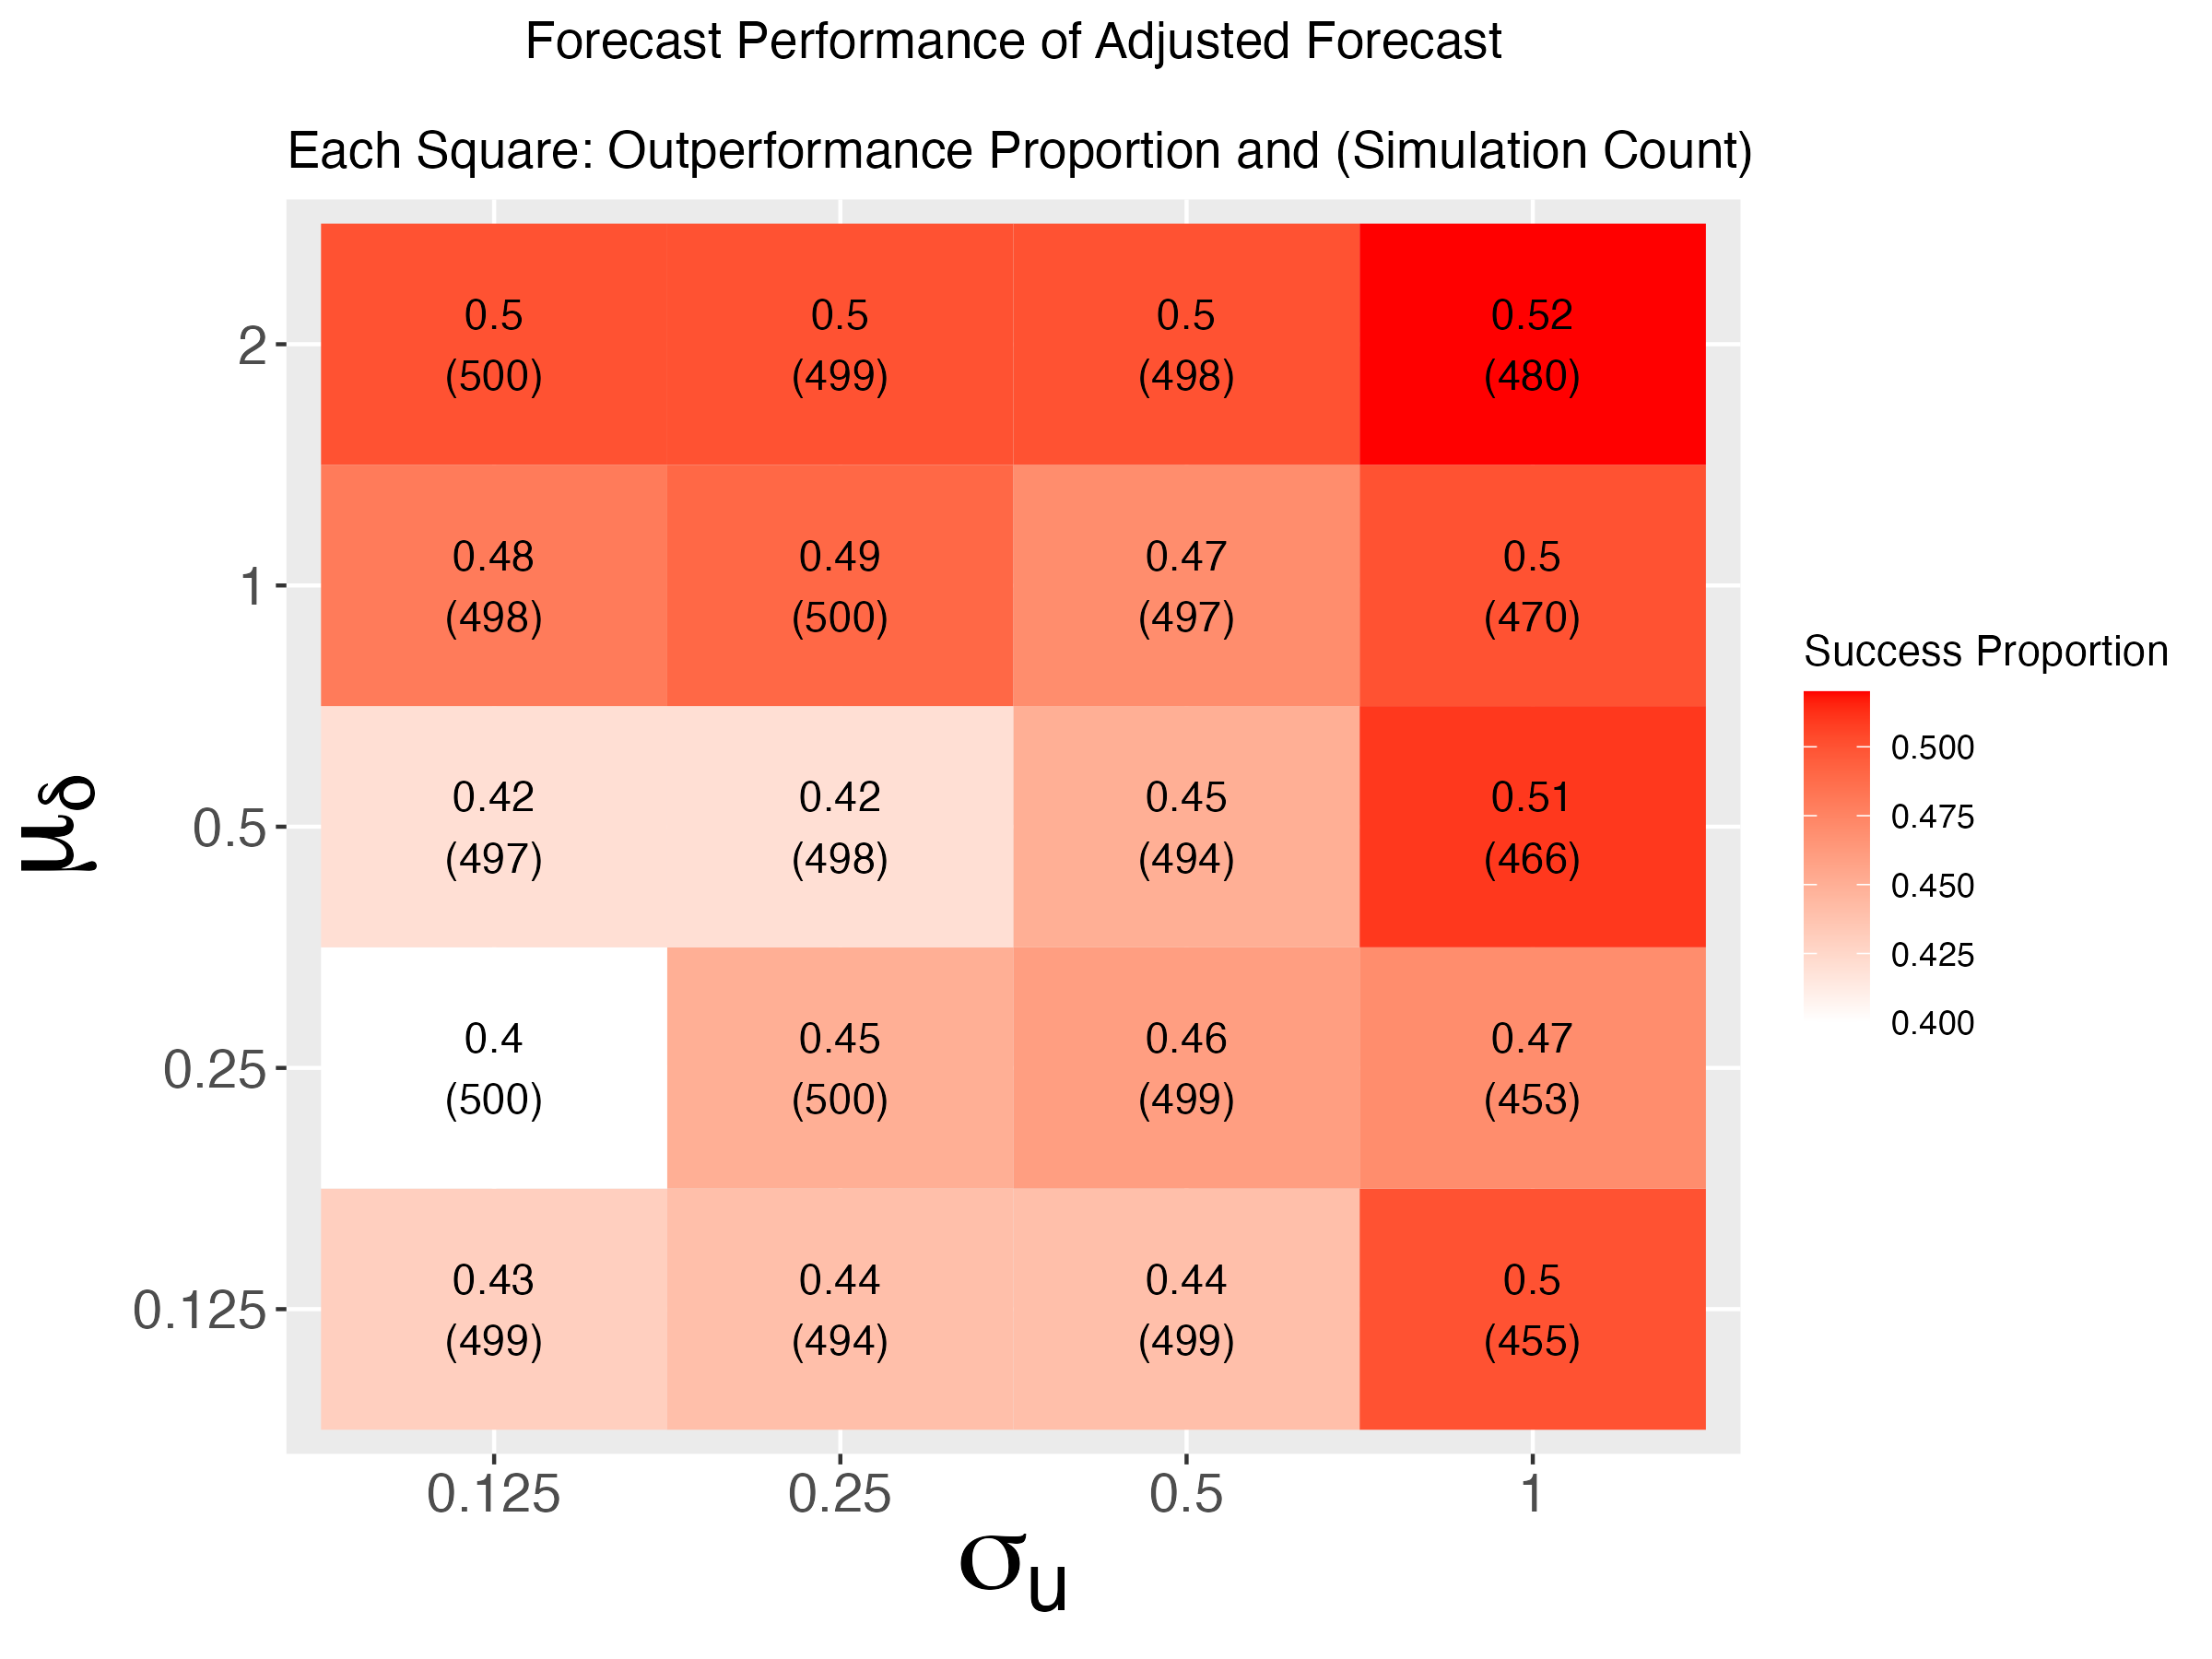
\includegraphics[scale = .42]{simulation_plots/Aug28_224311_2024_mu[delta]_sigma[u].png}
        \caption{Fixed values: $\mu_{v} = .125, \sigma_{v} = .125, \mu_{\omega^{*}} = .125$}\label{fig:sim_1}
    \end{subfigure}\hspace{12mm} %
    \begin{subfigure}{.44\linewidth} 
      \centering
        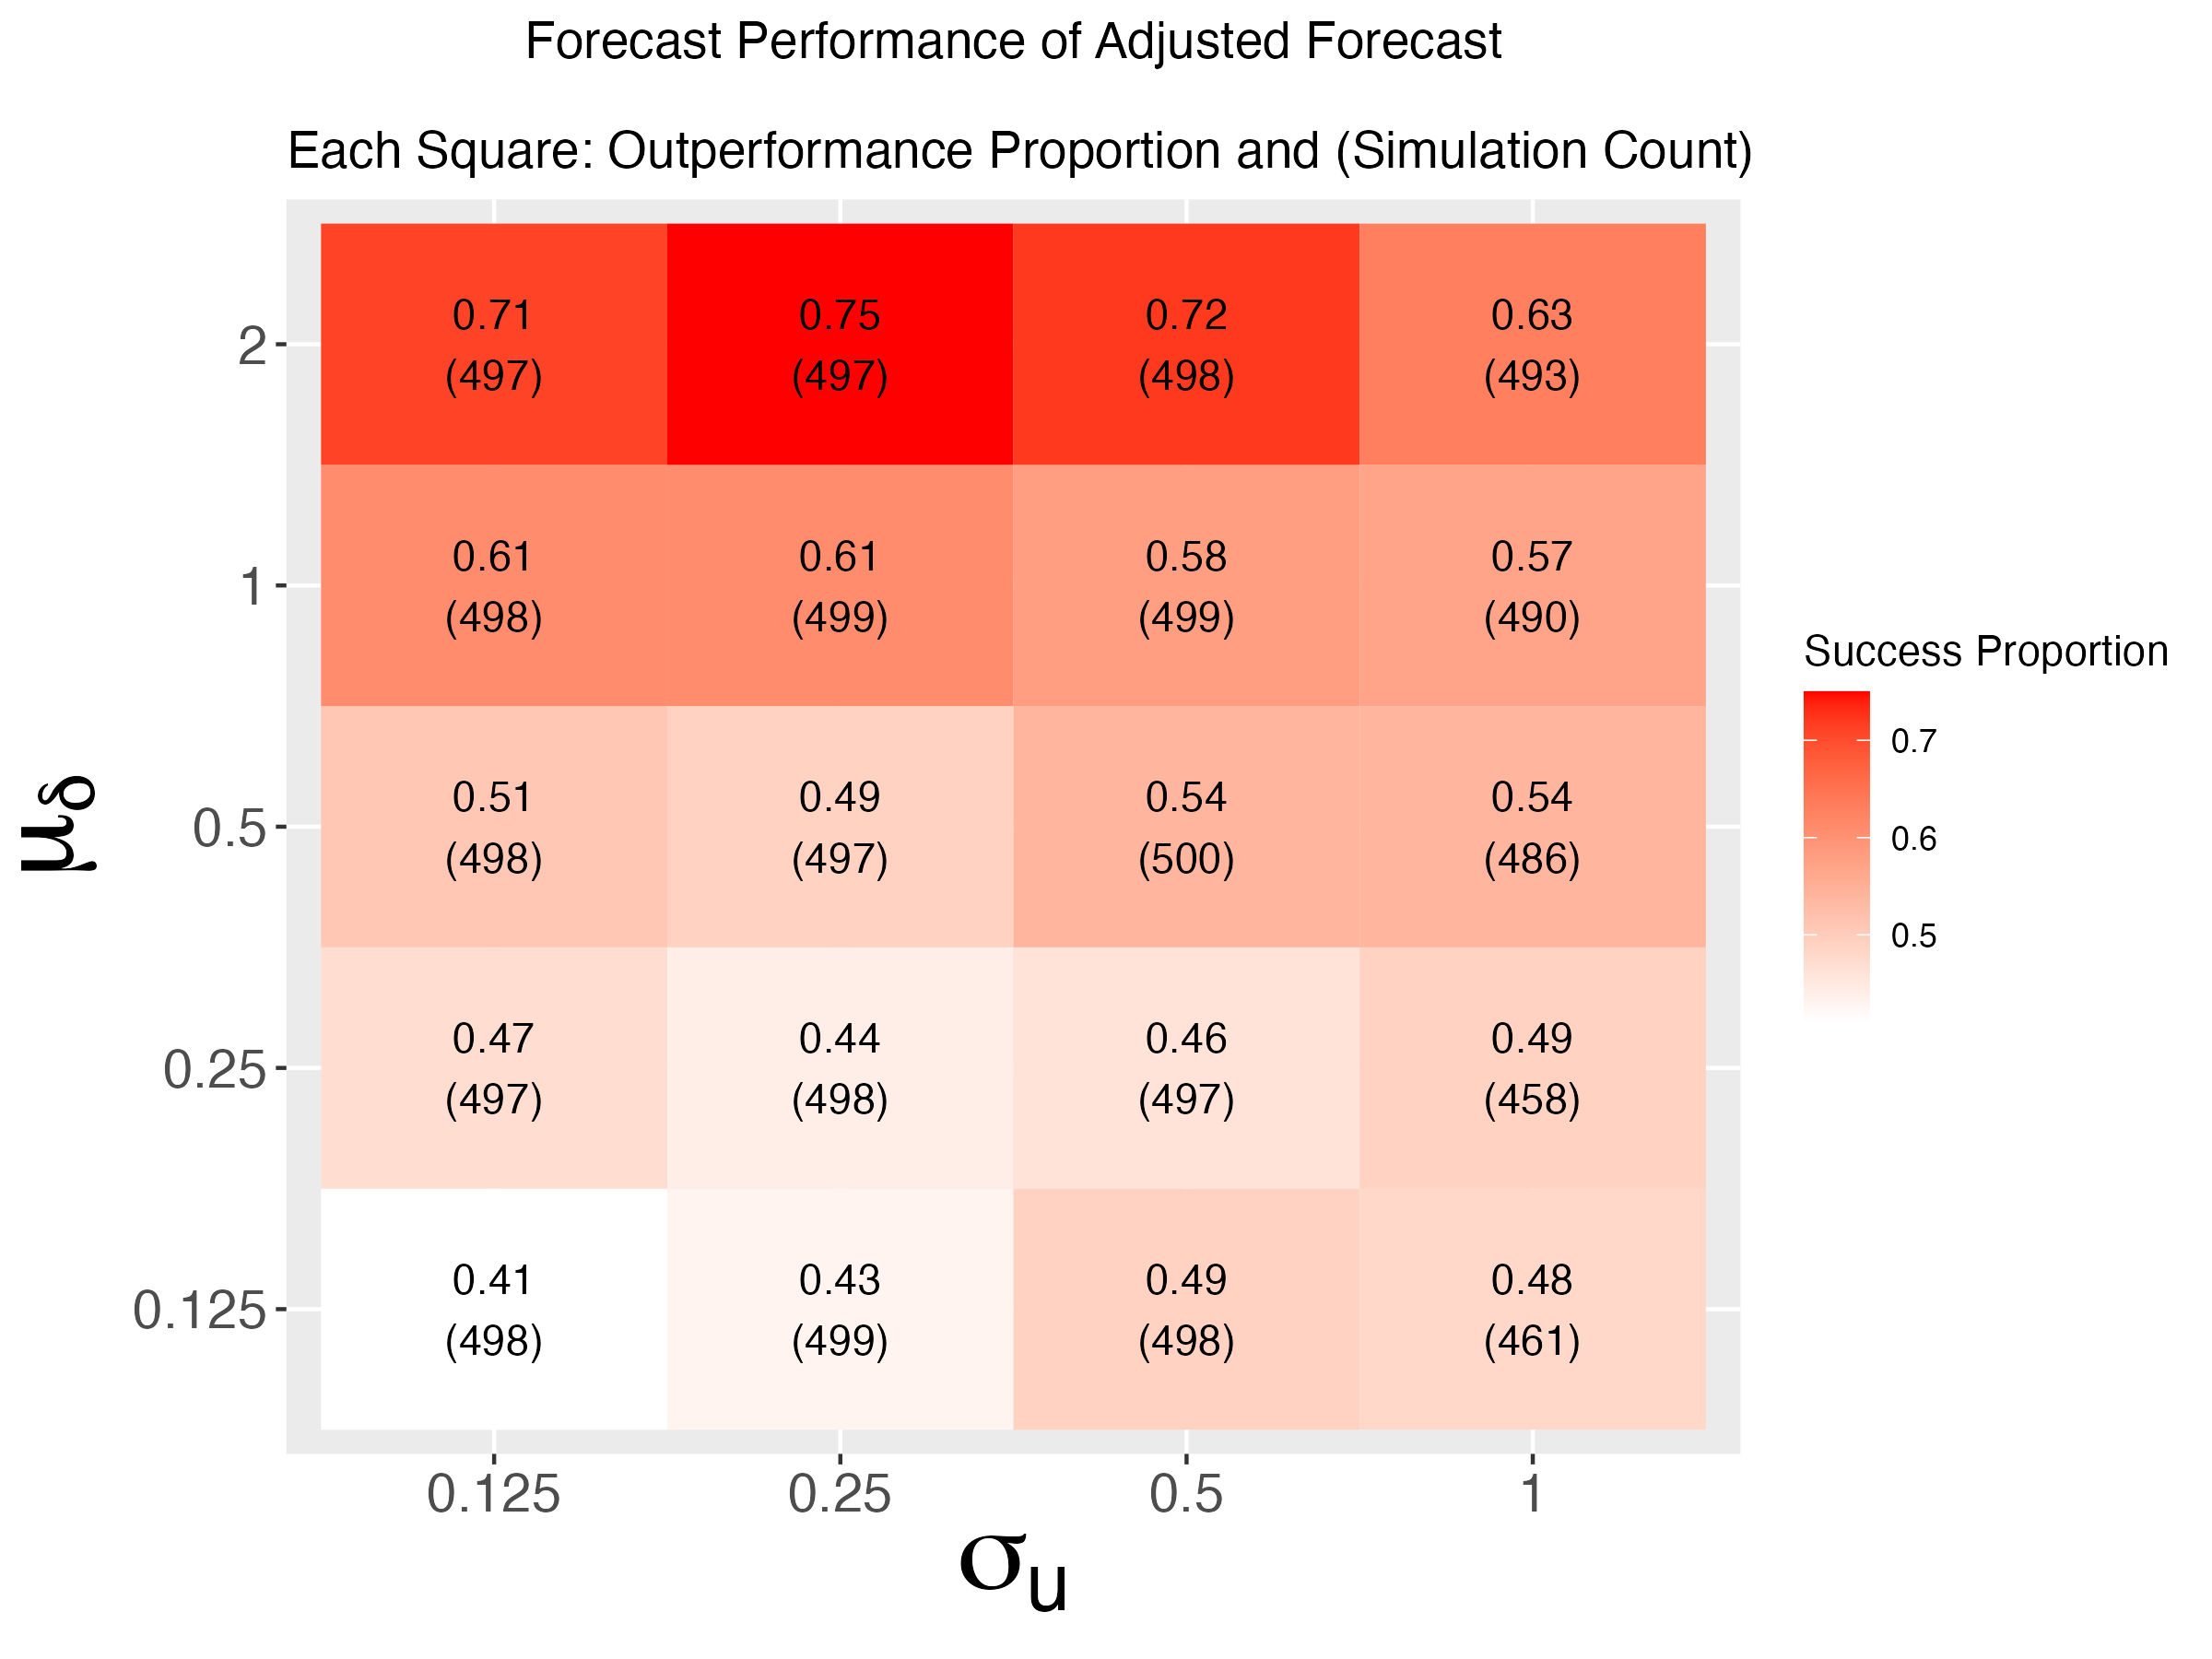
\includegraphics[scale=.42]{simulation_plots/Aug28_224317_2024_mu[delta]_sigma[u].png}
        \caption{Fixed values: $\mu_{v} = .5, \sigma_{v} = .125, \mu_{\omega^{*}} = .125$}\label{fig:sim_2}
    \end{subfigure}

    \begin{subfigure}{.44\linewidth} 
      \centering
        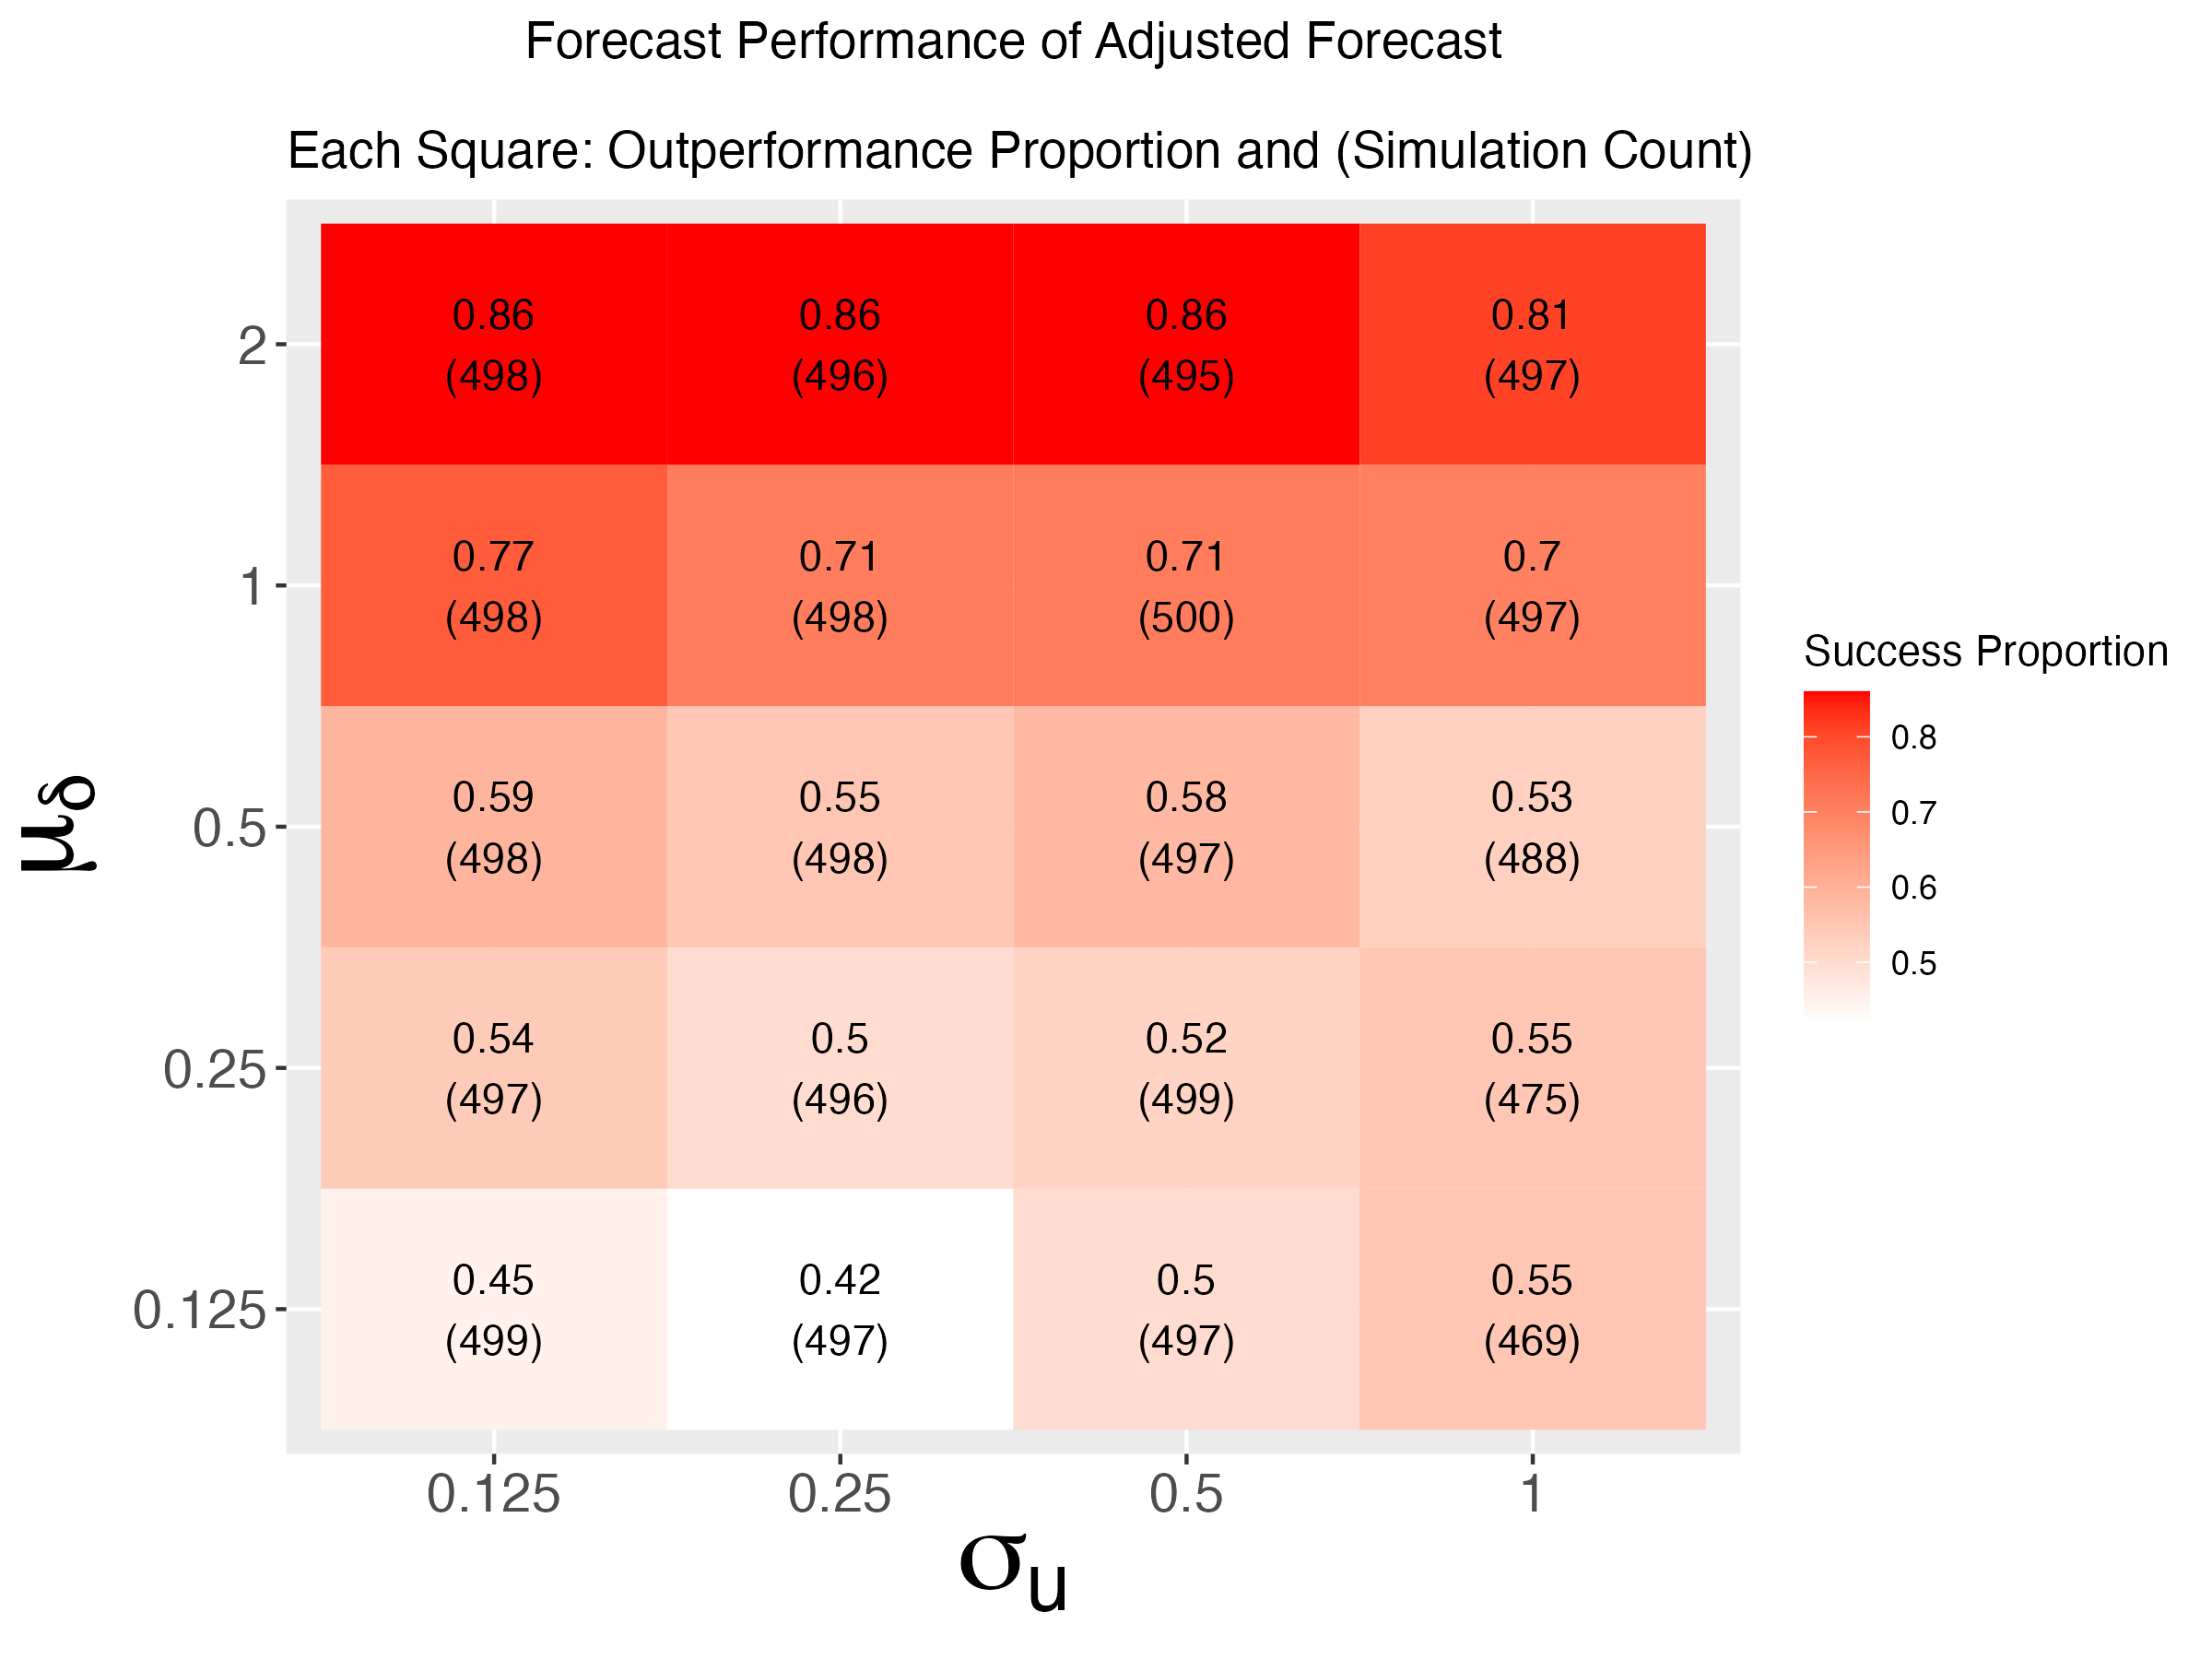
\includegraphics[scale=.42]{simulation_plots/Aug28_224322_2024_mu[delta]_sigma[u].png}
        \caption{Fixed values: $\mu_{v} = 1, \sigma_{v} = .125, \mu_{\omega^{*}} = .125$}\label{fig:sim_3}
    \end{subfigure}
    
        \caption{In the progression from \ref{fig:sim_1} to \ref{fig:sim_2} to \ref{fig:sim_3}, we see that increasing $\mu_{\delta}$ leads to improved performance of the adjusted forecast, and this effect is intensified as $\mu_{v}$ increases.  However, it is not consistently true that an increasing noise undermines the performance of the adjusted forecast.  Rather, that phenomenon requires both large quantites of $\mu_{\delta}$ and $\mu_{v}$.}
        \label{fig:signoise}
      \end{figure}

  \begin{figure}[!h]
    \centering
    \textbf{Interaction between Signal and Volatility Profile Means}\par\medskip
  \begin{subfigure}{.44\linewidth} 
    \centering
      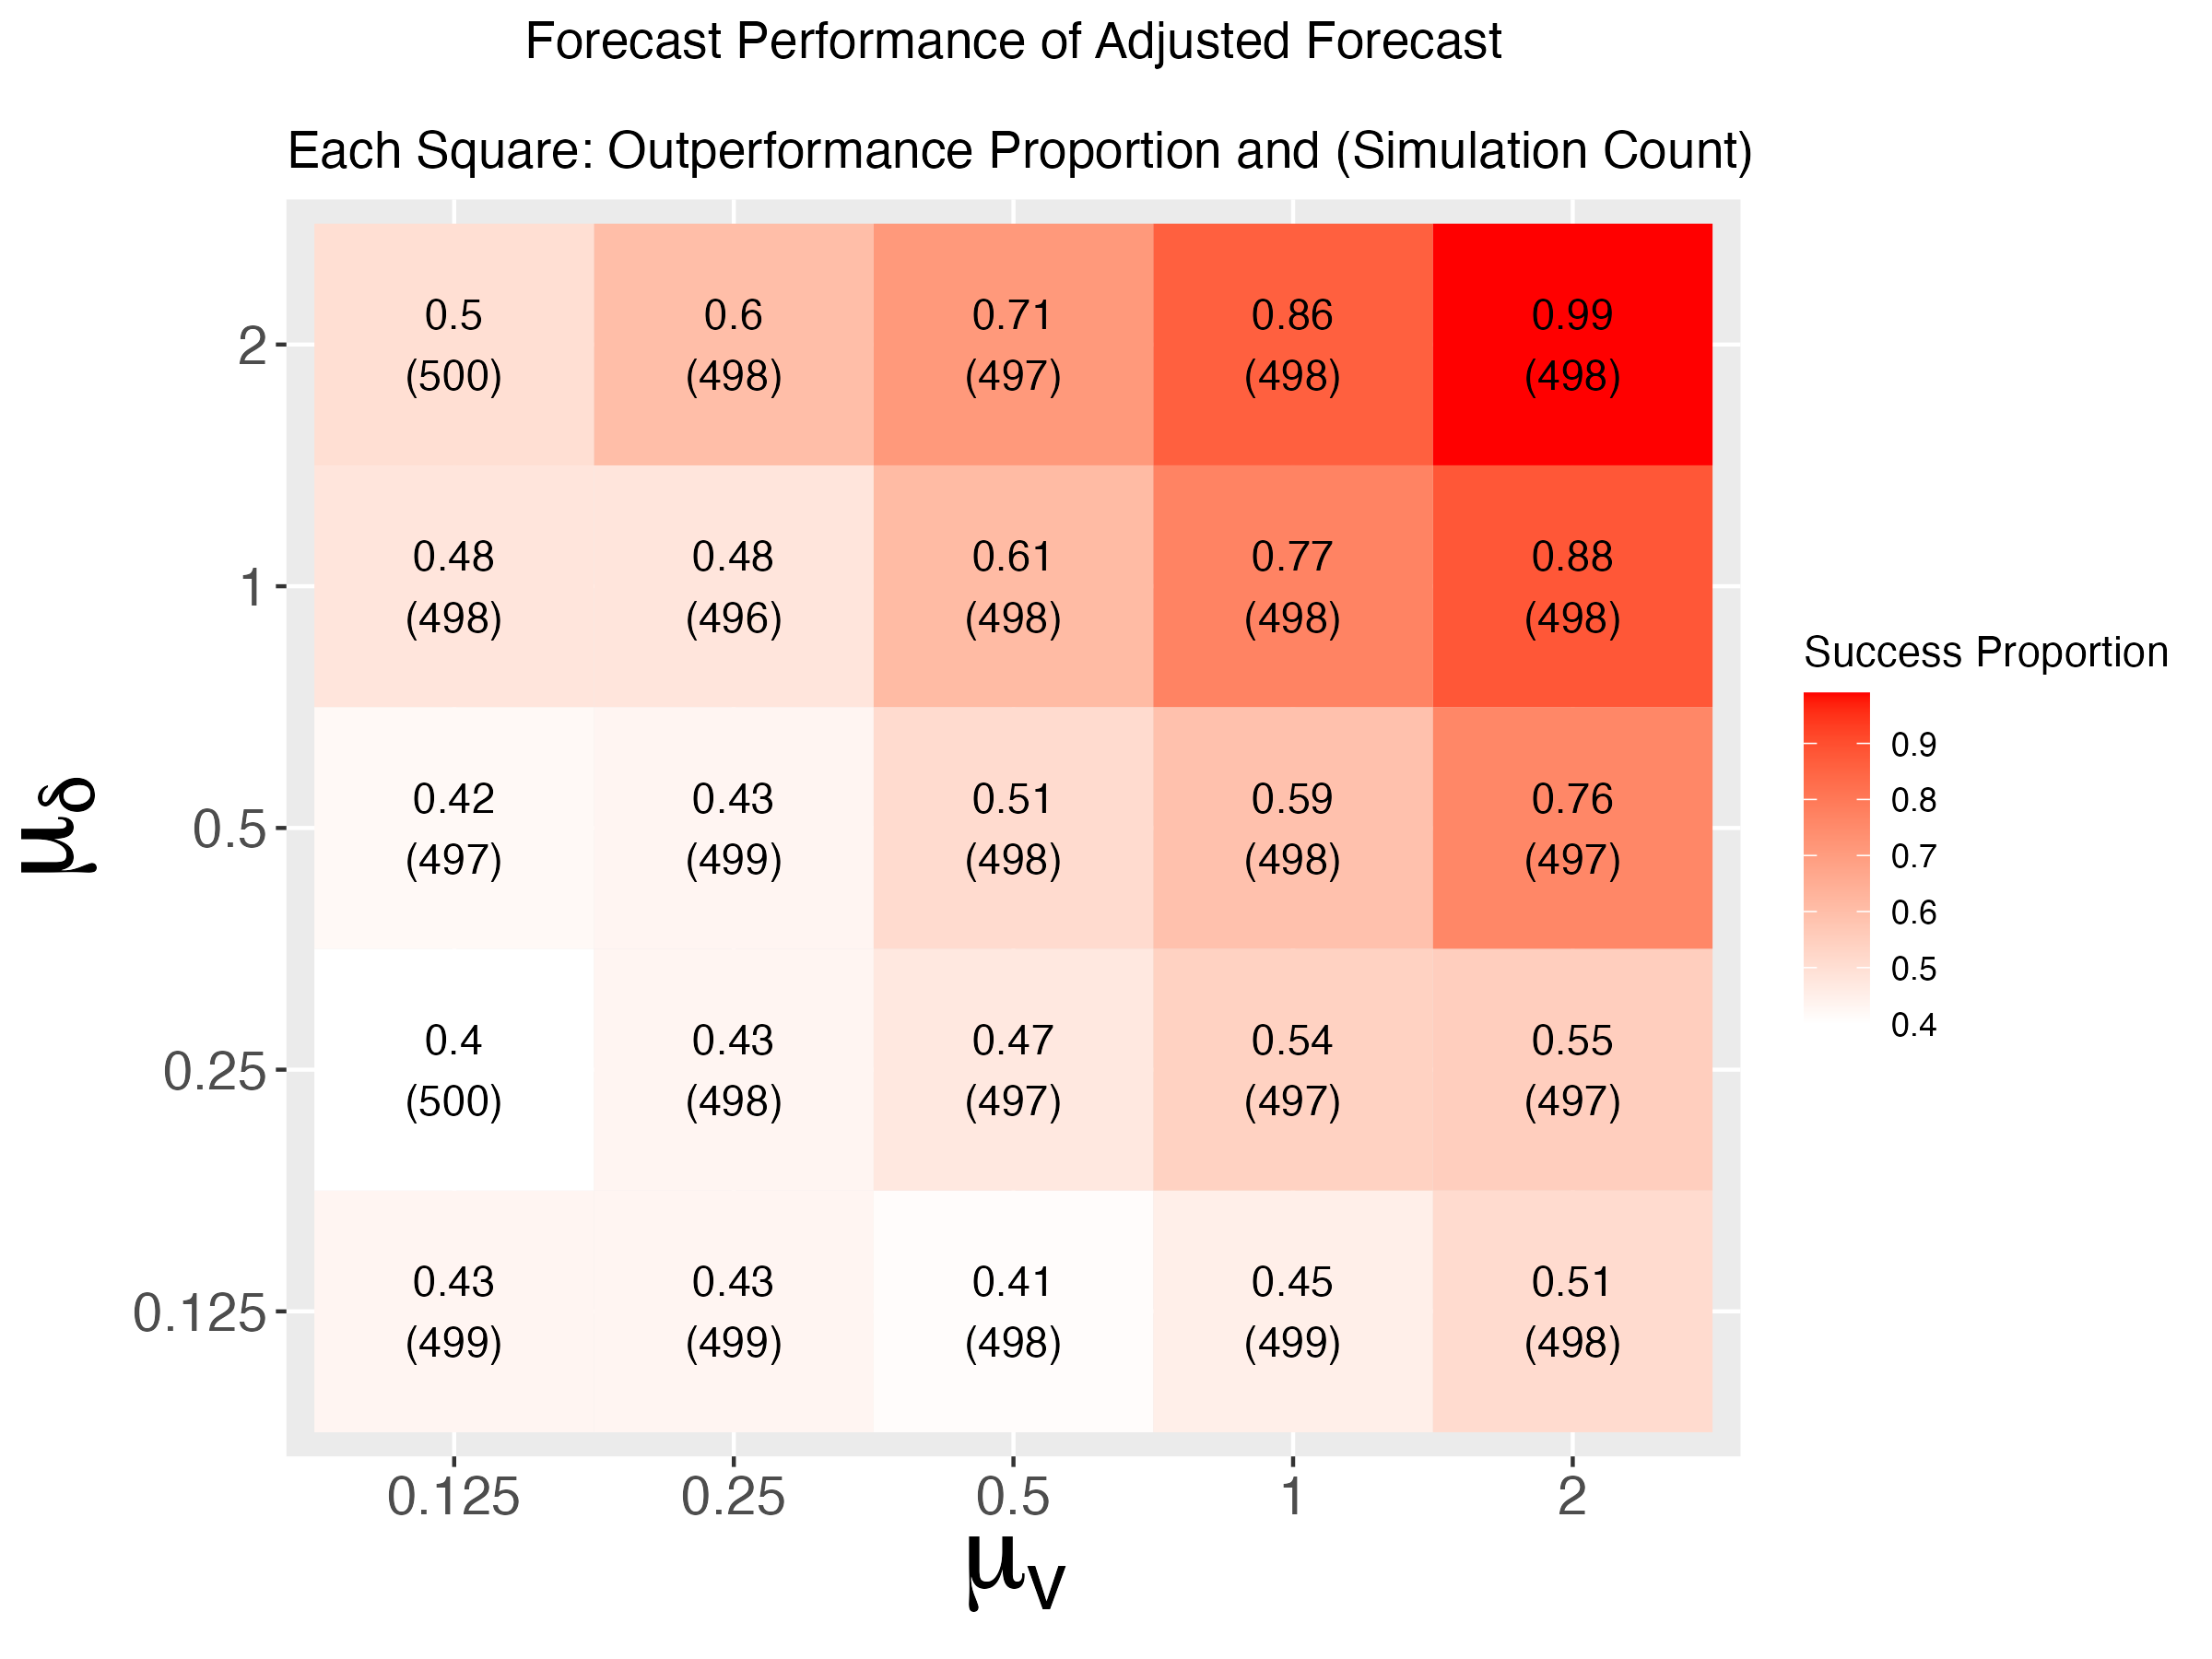
\includegraphics[scale = .42]{simulation_plots/Aug28_224330_2024_mu[delta]_mu[v].png}
      \caption{Fixed values: $\sigma_{v} = .125, \mu_{\omega^{*}} = .125, \sigma_{u} = .125$}\label{fig:sim_4}
  \end{subfigure}\hspace{12mm} %
  \begin{subfigure}{.44\linewidth} 
    \centering
      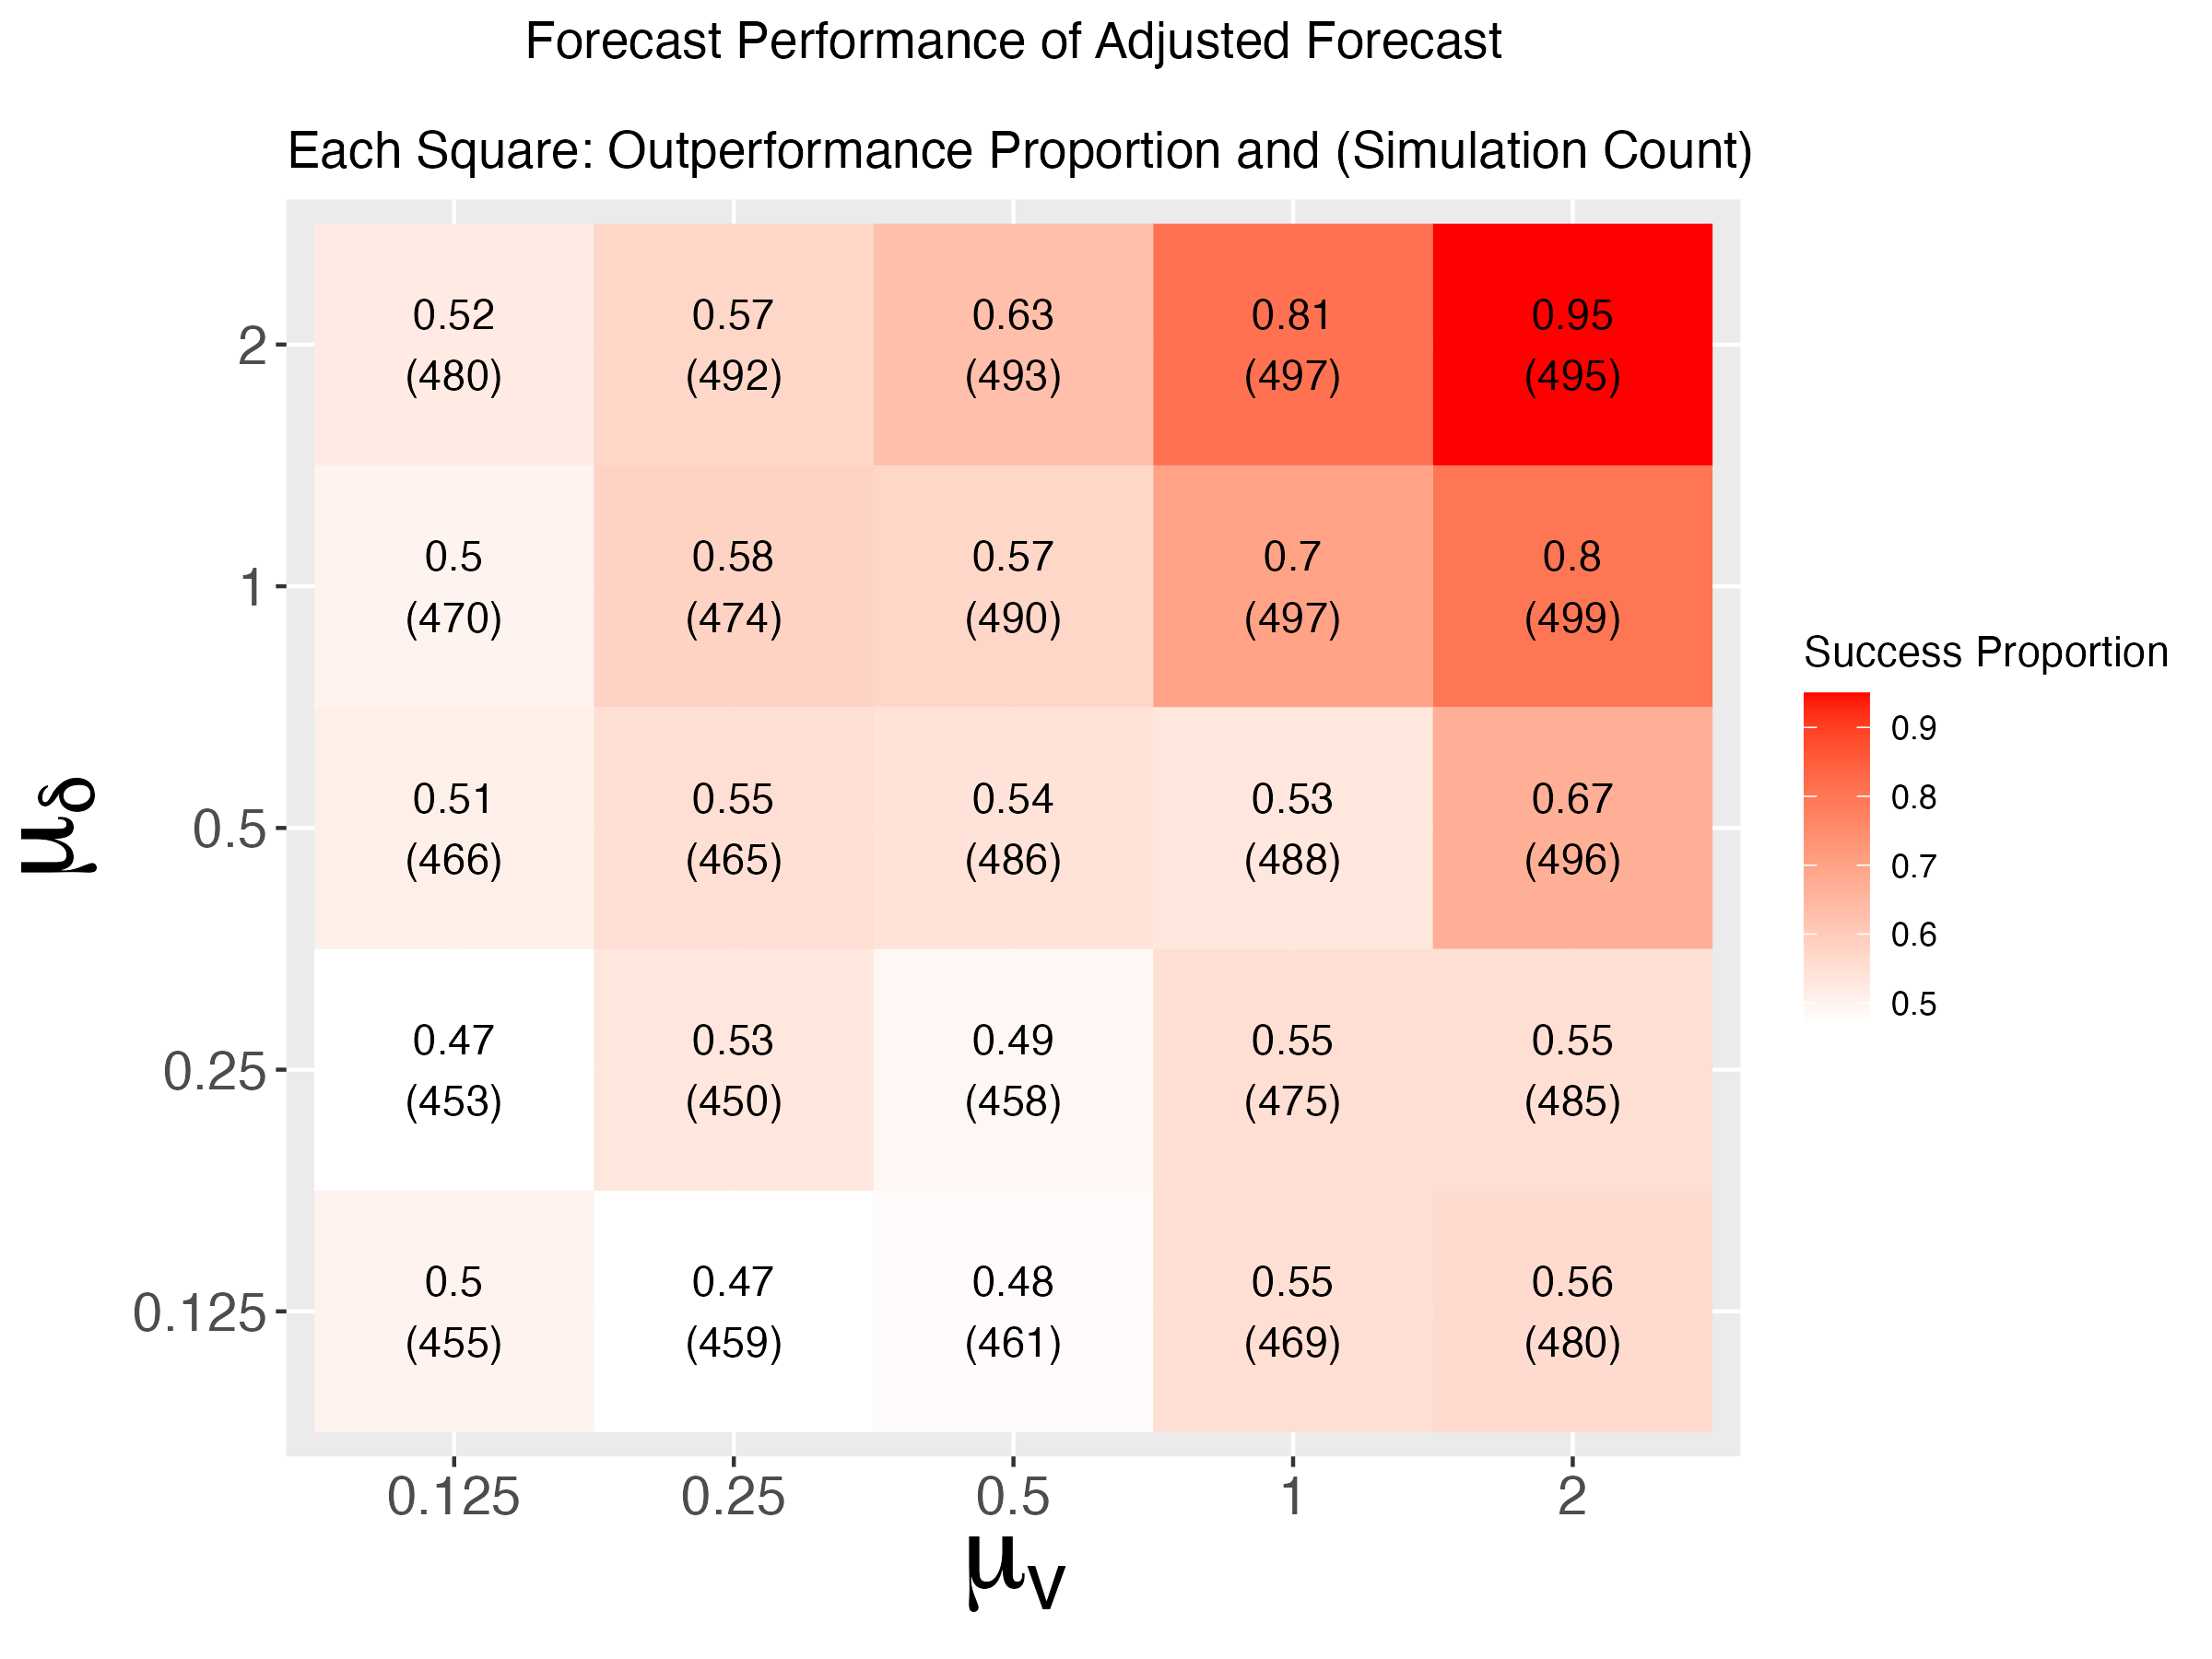
\includegraphics[scale=.42]{simulation_plots/Aug28_224337_2024_mu[delta]_mu[v].png}
      \caption{Fixed values: $\sigma_{v} = .125, \mu_{\omega^{*}} = .125, \sigma_{u} = 1$}\label{fig:sim_5}
  \end{subfigure}
  
      \caption{We compare the interaction of $\mu_{\delta}$ and $\mu_{v}$ at two different levels of shock noise.  In the low-noise regime, the peak performance of the adjusted forecast is higher, and the ascent is faster along both dimensions.   However, in the high-noise regime, the adjusted forecast performs well even at low levels of $\mu_{\delta}$ and $\mu_{v}$.}
      \label{fig:sig_volprof}
    \end{figure}

\begin{figure}[!h]
  \centering
  \textbf{Interaction between Shock Intercept and Shock Noise}\par\medskip
\begin{subfigure}{.44\linewidth} 
  \centering
    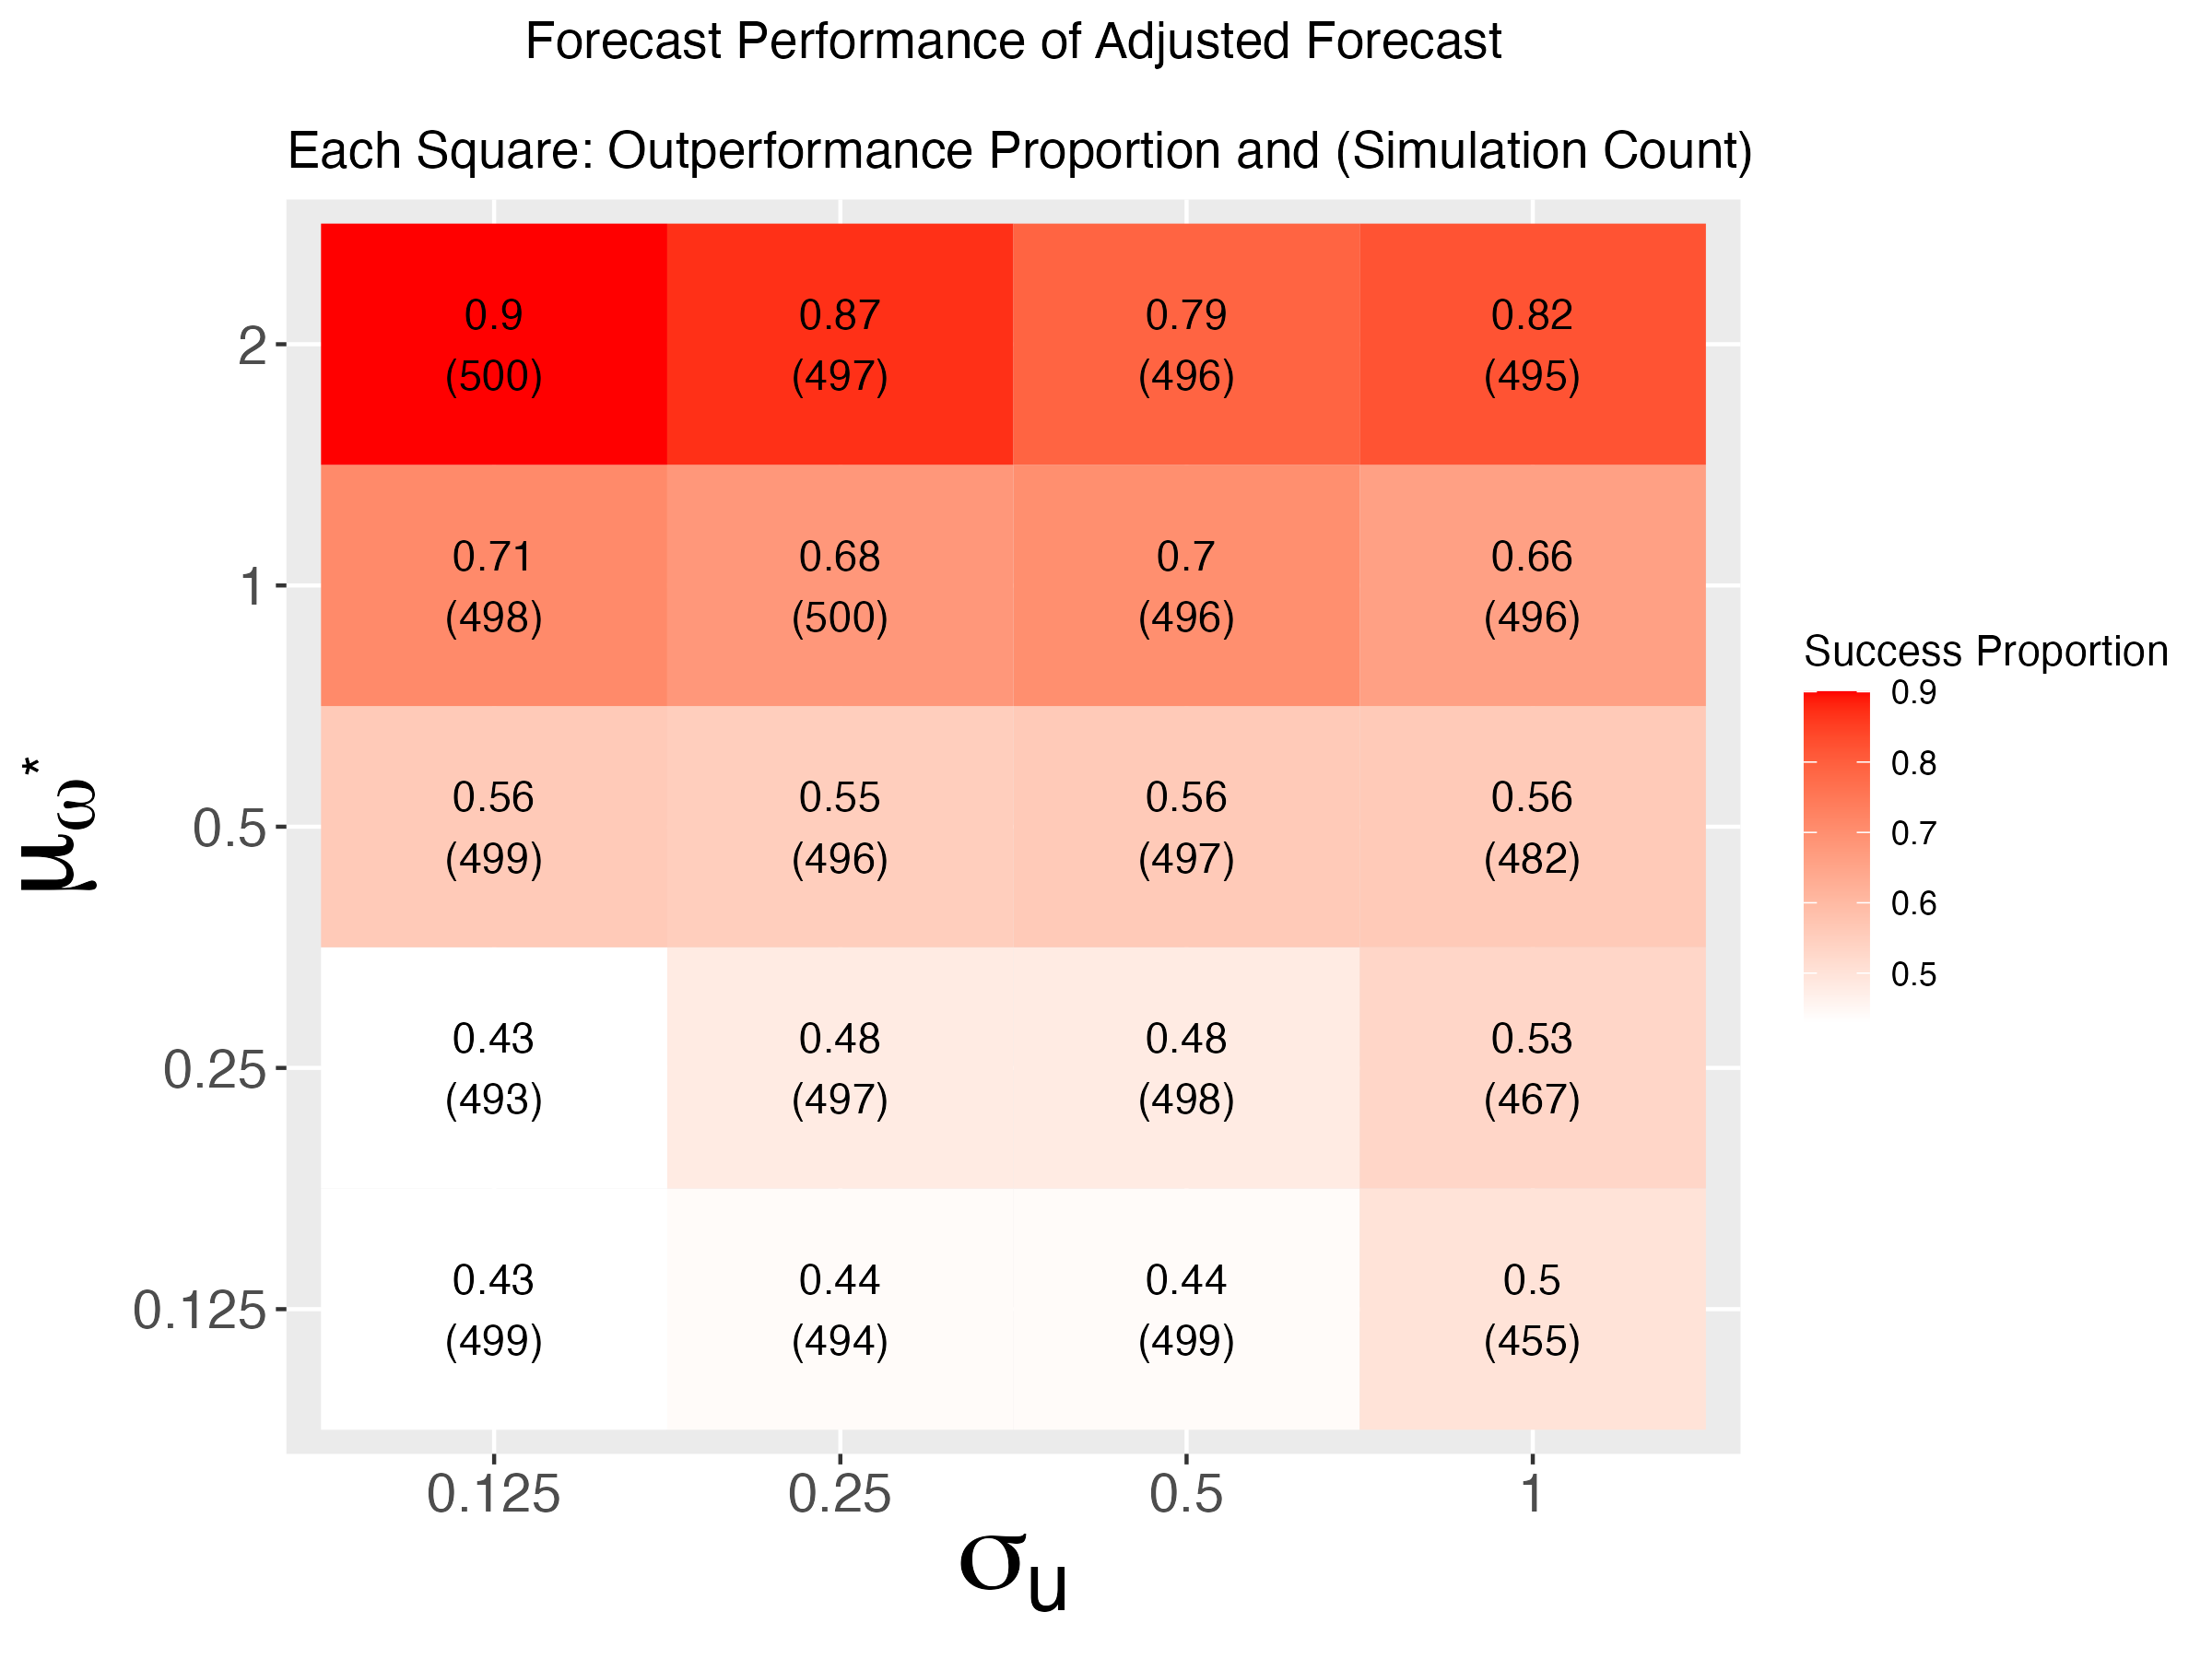
\includegraphics[scale = .42]{simulation_plots/Aug28_224451_2024_mu[omega^*]_sigma[u].png}
    \caption{Fixed values: $\mu_{v} = .125, \sigma_{v} = .125, \delta = .125$}\label{fig:sim_6}
\end{subfigure}\hspace{12mm} %
\begin{subfigure}{.44\linewidth} 
  \centering
    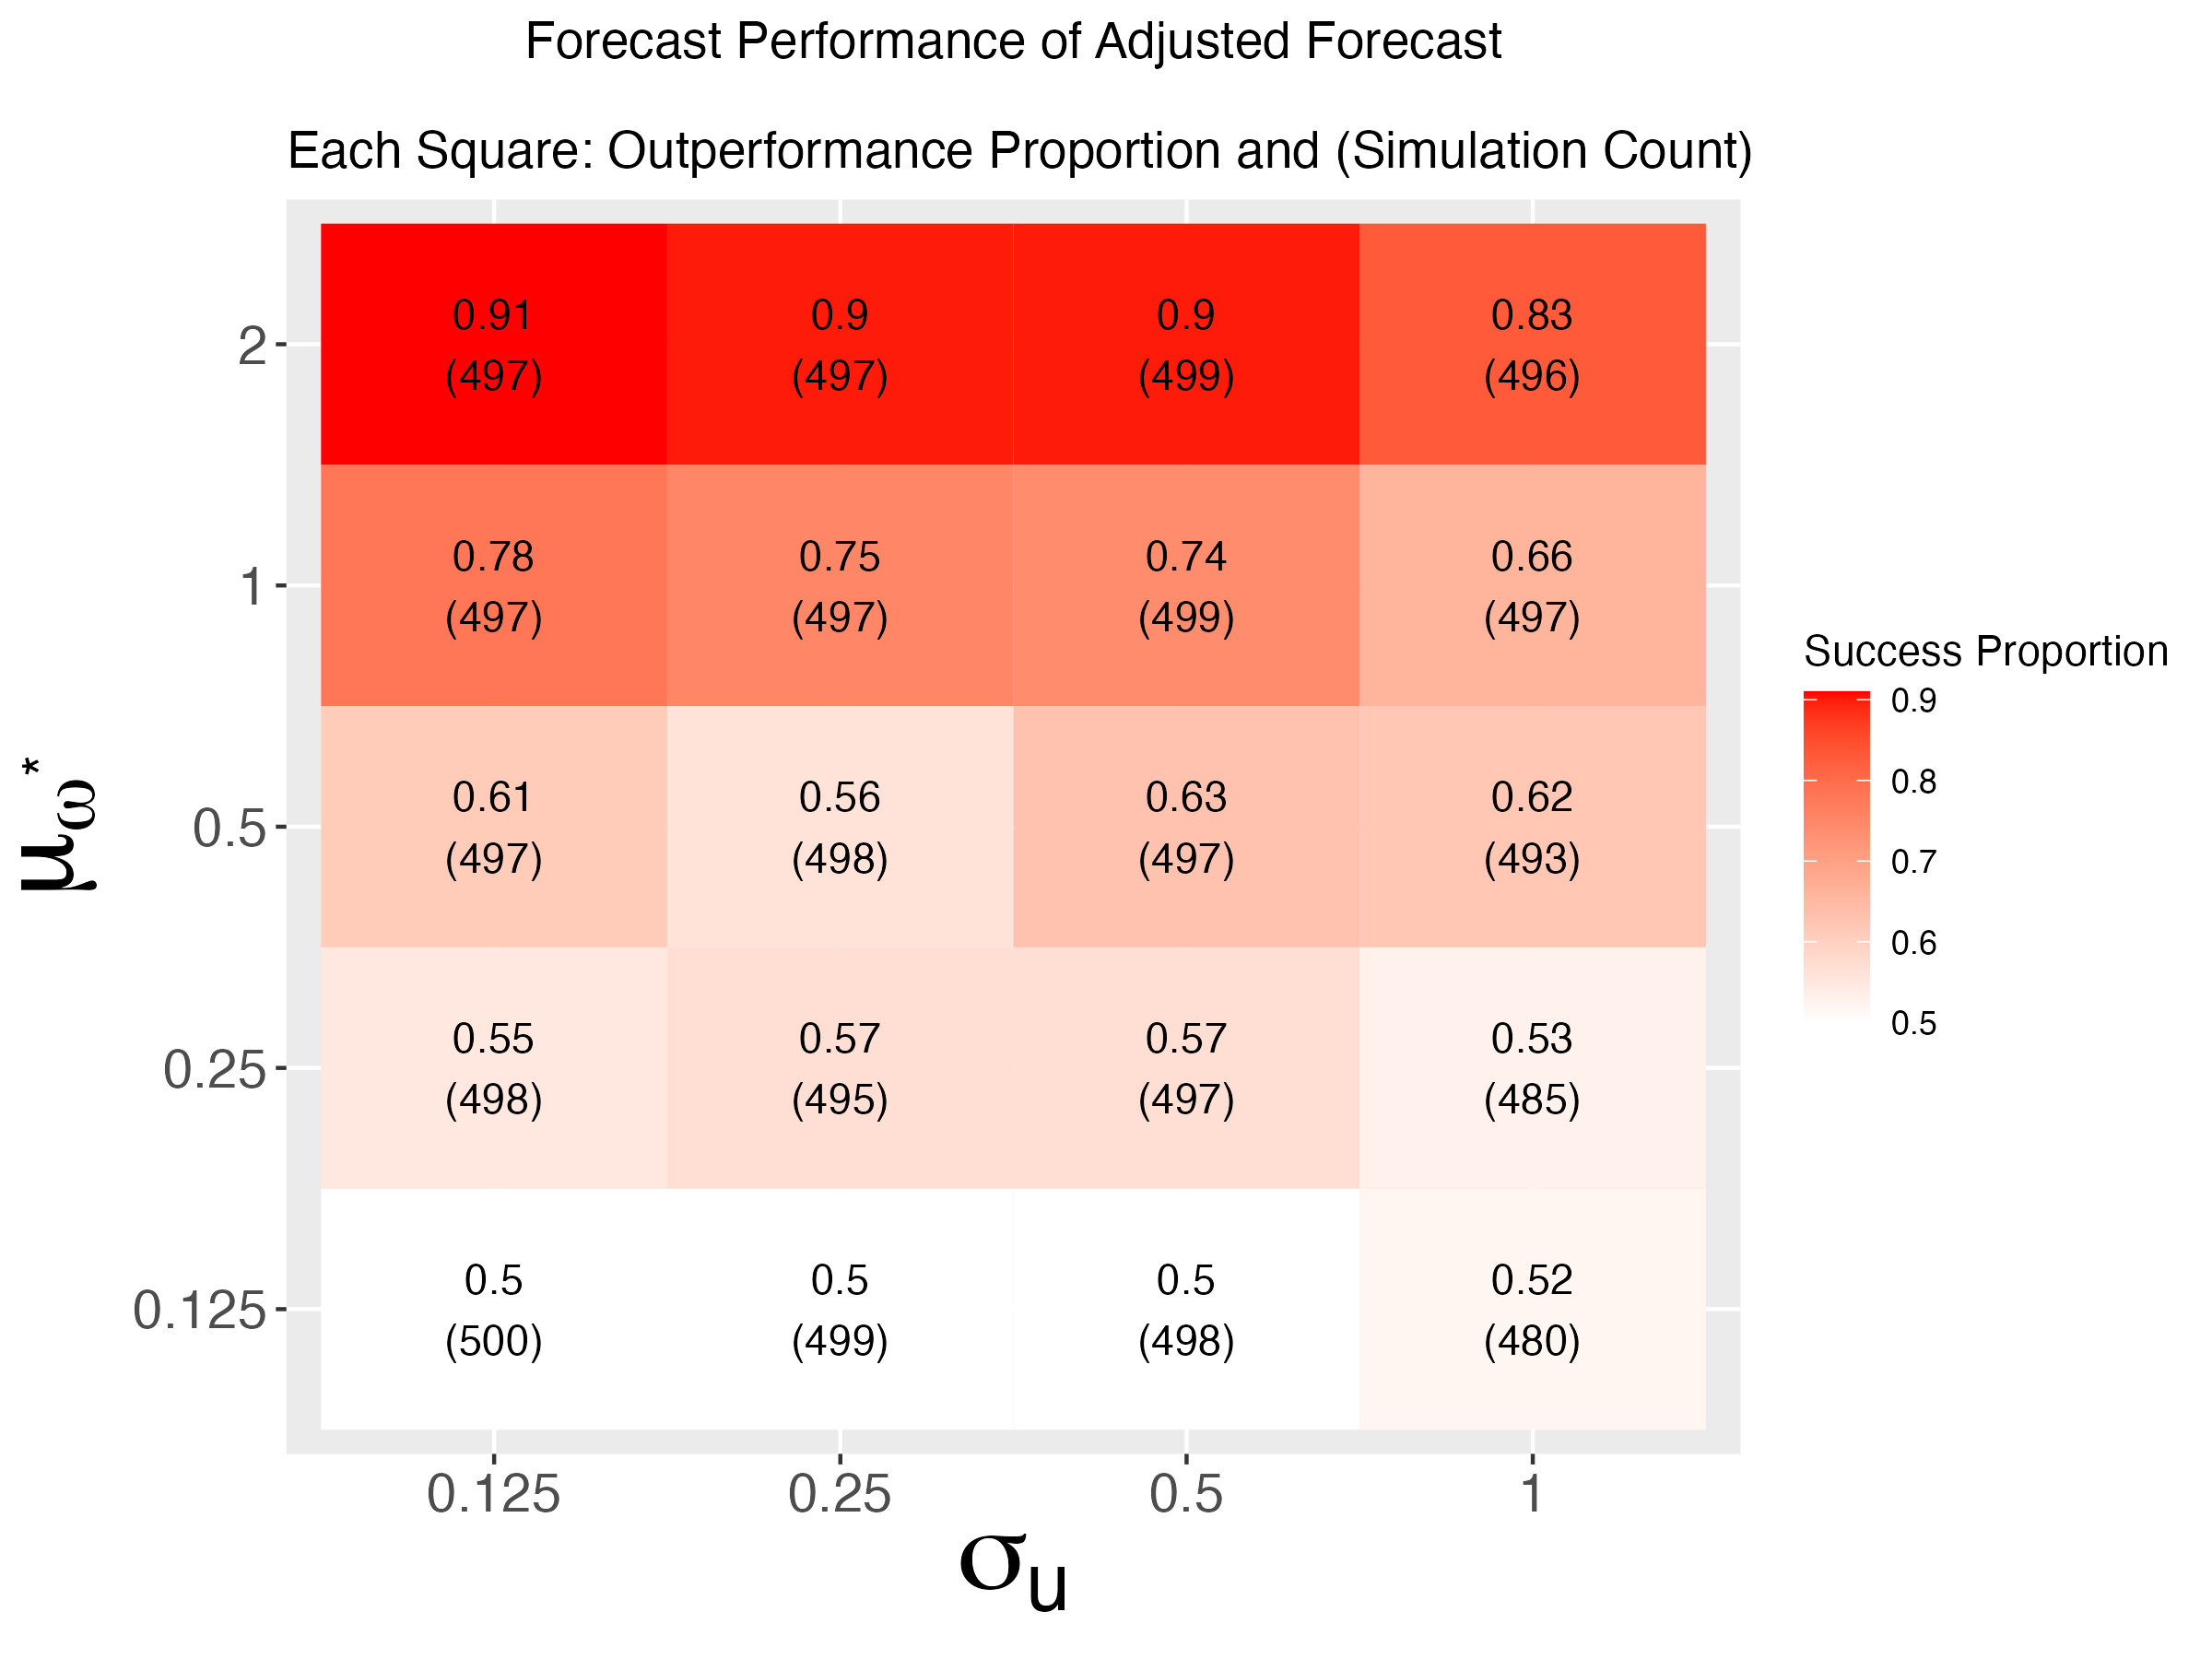
\includegraphics[scale=.42]{simulation_plots/Aug28_224455_2024_mu[omega^*]_sigma[u].png}
    \caption{Fixed values: $\mu_{v} = .125, \sigma_{v} = .125, \delta = 2$}\label{fig:sim_7}
\end{subfigure}

    \caption{The interaction between the intercept $\mu_{\omega^{*}}$ and $\sigma_{u}$ suggests that the parameters behave as expected.  However, a larger value of $\delta$ in \ref{fig:sim_7} attenuates the effect of increasing noise.}
    \label{fig:intercept_noise}
  \end{figure}

\clearpage 

\chapter{Conclusion}

We begin by recalling two salient quotes from important figures in the econometrics and forecasting literature:

\begin{quote}
  [There exists] conflict between the intuitive notion that more relevant information should help in forecasting, and the hard reality that attempts to make it do so have not been uniformly successful \parencite[][]{clements2005guest}
\end{quote}

\begin{quote}
incomplete information by itself is unlikely to play a key role in forecast failure (except if that information would forecast breaks). Consequently, using large amounts of data may not correct one of the main problems confronting forecasters, namely location shifts, unless that additional information is directly pertinent to forecasting breaks \parencite[][]{castle2013forecasting}
\end{quote}


% per Graduate College preference, place the \appendix and the appendices content before the
% bibliography (here) only if the appendices contain references.

\backmatter

\printbibliography[heading=bibintoc,title={References}]

% the below lines are only needed if bibliography precedes appendices
% uses https://tex.stackexchange.com/a/440212 to continue page numbering
\clearpage
\setcounter{counterforappendices}{\value{page}}
\mainmatter
\setcounter{page}{\value{counterforappendices}}

% \appendix

% \chapter{An appendix}


% \input{Appendix.tex}

\end{document}
